\documentclass[12pt]{report}

% includes
\usepackage{listings}           % for inline code
\usepackage{geometry}           % page size
\usepackage[utf8]{inputenc}     % encoding
\usepackage{palatino}           % font
\usepackage[english]{babel}     % language
\usepackage{graphicx}           % images
\usepackage{indentfirst}        % indentation
\usepackage[nottoc]{tocbibind}  % table of contents style
\usepackage[unicode]{hyperref}  % references from the table of contents
\usepackage{xcolor}             % to define colors
\usepackage{wrapfig}

\setcounter{tocdepth}{4}
\setcounter{secnumdepth}{3}

% Copyright 2017 Sergei Tikhomirov, MIT License
% https://github.com/s-tikhomirov/solidity-latex-highlighting/

\usepackage{listings, xcolor}

\definecolor{verylightgray}{rgb}{.97,.97,.97}

\lstdefinelanguage{Solidity}{
	keywords=[1]{anonymous, assembly, assert, balance, break, call, callcode, case, catch, class, constant, continue, leave, constructor, contract, debugger, default, delegatecall, delete, do, else, emit, event, experimental, export, external, false, finally, for, function, gas, if, implements, import, in, indexed, instanceof, interface, internal, is, length, library, log0, log1, log2, log3, log4, memory, modifier, new, payable, pragma, private, protected, public, pure, push, require, return, returns, revert, selfdestruct, invalid, send, solidity, storage, struct, suicide, super, switch, then, this, throw, transfer, true, try, typeof, using, value, view, while, with, addmod, ecrecover, keccak256, mulmod, ripemd160, sha256, sha3}, % generic keywords including crypto operations
	keywordstyle=[1]\color{blue}\bfseries,
	keywords=[2]{address, bool, byte, bytes, bytes1, bytes2, bytes3, bytes4, bytes5, bytes6, bytes7, bytes8, bytes9, bytes10, bytes11, bytes12, bytes13, bytes14, bytes15, bytes16, bytes17, bytes18, bytes19, bytes20, bytes21, bytes22, bytes23, bytes24, bytes25, bytes26, bytes27, bytes28, bytes29, bytes30, bytes31, bytes32, enum, int, int8, int16, int24, int32, int40, int48, int56, int64, int72, int80, int88, int96, int104, int112, int120, int128, int136, int144, int152, int160, int168, int176, int184, int192, int200, int208, int216, int224, int232, int240, int248, int256, mapping, string, uint, uint8, uint16, uint24, uint32, uint40, uint48, uint56, uint64, uint72, uint80, uint88, uint96, uint104, uint112, uint120, uint128, uint136, uint144, uint152, uint160, uint168, uint176, uint184, uint192, uint200, uint208, uint216, uint224, uint232, uint240, uint248, uint256, var, void, ether, finney, szabo, wei, days, hours, minutes, seconds, weeks, years},	% types; money and time units
	keywordstyle=[2]\color{teal}\bfseries,
	keywords=[3]{block, blockhash, coinbase, difficulty, gaslimit, number, timestamp, msg, data, gas, sender, sig, value, now, tx, gasprice, origin},	% environment variables
	keywordstyle=[3]\color{violet}\bfseries,
	identifierstyle=\color{black},
	sensitive=false,
	comment=[l]{//},
	morecomment=[s]{/*}{*/},
	commentstyle=\color{gray}\ttfamily,
	stringstyle=\color{red}\ttfamily,
	morestring=[b]',
	morestring=[b]"
}

\lstset{
	language=Solidity,
	backgroundcolor=\color{verylightgray},
	extendedchars=true,
	basicstyle=\footnotesize\ttfamily,
	showstringspaces=false,
	showspaces=false,
	numbers=left,
	numberstyle=\footnotesize,
	numbersep=9pt,
	tabsize=2,
	breaklines=true,
	showtabs=false,
	captionpos=b
}	% for solidity highlighting



% includes options
\geometry{  a4paper,            % scientific thesis standard
            left=3cm,
            right=2cm,
            top=2cm,
            bottom=2cm,
 }
\graphicspath{{images/}}        % path where the images are located
\setlength{\parindent}{1cm}     % paragraph indentation

% other options
\linespread{1.5}                % space between lines
\renewcommand*\contentsname{Cuprins}    % table of contents name

\setlength{\parindent}{1cm}     % paragraph indentation

\definecolor{codegreen}{rgb}{0,0.6,0}
\definecolor{codegray}{rgb}{0.5,0.5,0.5}
\definecolor{codepurple}{rgb}{0.58,0,0.82}
\definecolor{backcolour}{rgb}{0.95,0.95,0.92}
\lstdefinestyle{mystyle}{
    backgroundcolor=\color{backcolour},   
    commentstyle=\color{codegreen},
    keywordstyle=\color{magenta},
    numberstyle=\tiny\color{codegray},
    stringstyle=\color{codepurple},
    basicstyle=\ttfamily\footnotesize,
    breakatwhitespace=false,         
    breaklines=true,                 
    captionpos=b,                    
    keepspaces=true,                 
    numbers=left,                    
    numbersep=5pt,                  
    showspaces=false,                
    showstringspaces=false,
    showtabs=false,                  
    tabsize=2,
}
\lstset{style=mystyle}


% the document content
\begin{document}
    % macros (global)
    \newcommand{\university}    {"Alexandru-Ioan Cuza" University, Iași}
\newcommand{\universityg}   {"Alexandru-Ioan Cuza" University, Iași} % genitive
\newcommand{\faculty}       {Faculty of Computer Science}
\newcommand{\facultyg}      {Faculty of Computer Science} % genitive
\newcommand{\speciality}    {computer science}
\newcommand{\promotion}     {2022}                                  %<---------

\newcommand{\thesistype}    {Master's Thesis}
\newcommand{\thesistitle}   {Solidity Optimization using Control Flow Graphs}    %<---------

\newcommand{\authorlast}    {Iacob}                               %<---------
\newcommand{\authorfirst}   {Sergiu}
\newcommand{\authornamefl}  {\authorfirst \space \authorlast} % first name first
\newcommand{\authornamelf}  {\authorlast \space \authorfirst} % last name first
\newcommand{\authorbirth}   {01 March 1997}                      %<---------
\newcommand{\authoraddress} {România, jud. Iași, mun. Iași} %<---------
\newcommand{\authorcnp}     {-}                         %<---------

\newcommand{\session}       {july, 2022}                       %<---------
\newcommand{\coordinator}   {Dr. Arusoaie Andrei}               %<---------

\newcommand{\dottedline}    {............................}
    
    % front-matter
    \pagenumbering{gobble}
    
    % define the cover page
\begin{titlepage}
    \begin{center}
        % the university and faculty
        \large
        \MakeUppercase{\university}
        
        \LARGE
        \textbf{\MakeUppercase{\faculty}}
        
        % the faculty logo
        \vspace{1cm}
        
\includegraphics[width=0.3\textwidth]{logoFii.png}
        
        % thesis title
        \vspace{1cm}
        \Large
        \MakeUppercase{\thesistype}
        
        \vspace{0.5cm}
        \LARGE
        \textbf{\thesistitle}
        
        % author
        \vspace{2cm}
        \Large
        proposed by
        
        \vspace{0.5cm}
        \LARGE
        \textbf{\authornamelf}
        
        % session
        \vfill
        \Large
        \textbf{Session:} \session
        
        % scientific coordinator
        \vspace{2cm}
        \Large
        Scientific Coordinator
        
        \vspace{0.5cm}
        \LARGE
        \textbf{\coordinator}
    \end{center}
\end{titlepage}
    % define the title page
\begin{titlepage}
    \begin{center}
        % the university and faculty
        \large
        \MakeUppercase{\university}
        
        \LARGE
        \textbf{\MakeUppercase{\faculty}}
        
        % thesis title
        \vspace{8cm}
        \huge
        \textbf{\thesistitle}
        
        % author
        \vspace{2cm}
        \LARGE
        \textbf{\authornamefl}
        
        % session
        \vfill
        \Large
        \textbf{Session:} \session
        
        % scientific coordinator
        \vspace{4cm}
        \Large
        Coordinator
        
        \vspace{0.5cm}
        \LARGE
        \textbf{\coordinator}
    \end{center}
\end{titlepage}
    % \vspace*{\fill}

\begin{flushright}
    Avizat, \\
    Îndrumător lucrare de licență, \\
    \coordinator. \\
    Data: \dottedline \hspace{1cm} Semnătura: \dottedline
\end{flushright}

\vspace{1cm}
\begin{center}
    \large
    \textbf{Declarație privind originalitatea conținutului lucrării de licență}
\end{center}

Subsemnatul \textbf{\authornamelf} domiciliat în \textbf{\authoraddress}, născut la data de \textbf{\authorbirth}, identificat prin CNP \textbf{\authorcnp}, absolvent al \facultyg, \textbf{\faculty} specializarea \textbf{\speciality}, promoția \promotion, declar pe propria răspundere cunoscând consecințele falsului în declarații în sensul art. 326 din Noul Cod Penal și dispozițiile Legii Educației Naționale nr. 1/2011 art. 143 al. 4 și 5 referitoare la plagiat, că lucrarea de licență cu titlul \textbf{\thesistitle} elaborată sub îndrumarea domnului \textbf{\coordinator}, pe care urmează să o susțin în fața comisiei este originală, îmi aparține și îmi asum conținutul său în întregime.

De asemenea, declar că sunt de acord ca lucrarea mea de licență să fie verificată prin orice modalitate legală pentru confirmarea originalității, consimțind inclusiv la introducerea conținutului ei într-o bază de date în acest scop.

Am luat la cunoștință despre faptul că este interzisă comercializarea de lucrări științifice în vederea facilitării falsificării de către cumpărător a calității de autor al unei lucrări de licență, de diplomă sau de disertație și în acest sens, declar pe proprie răspundere că lucrarea de față nu a fost copiată ci reprezintă rodul cercetării pe care am întreprins-o.

\begin{flushright}
    Data: \dottedline \hspace{6cm} Semnătura: \dottedline
\end{flushright}

\vspace*{\fill}
\pagebreak
    % \vspace*{\fill}
\begin{center}
    \large
    \textbf{Declarație de consimțământ}
\end{center}

Prin prezenta declar că sunt de acord ca lucrarea de licență cu titlul \textbf{\thesistitle}, codul sursă al programelor și celelalte conținuturi (grafice, multimedia, date de test, etc.) care însoțesc această lucrare să fie utilizate în cadrul \facultyg.

De asemenea, sunt de acord ca \faculty \space de la \university, să utilizeze, modifice, reproducă și să distribuie în scopuri necomerciale programele-calculator, format executabil și sursă, realizate de mine în cadrul prezentei lucrări de licență.

\begin{flushright}
    Absolvent \textbf{\authornamefl} \\
    \vspace{0.5cm}
    Data: \dottedline \hspace{6cm} Semnătura: \dottedline
\end{flushright}
\vspace*{\fill}
\pagebreak
    
    % table of contents
    \tableofcontents
    
    \cleardoublepage
    % \phantomsection

    
    % \addcontentsline{toc}{chapter}{\listfigurename}
    \listoffigures

    % chapters
    \setcounter{page}{1}
    \pagenumbering{arabic}
    
    \chapter{Introduction} 
\section{Context}
\paragraph*{}
Static analysis has been at the core of \textbf{optimizing} code for many years now, doubled by its sibling, dynamic analysis. Common programming languages such as C++, Java, Golang etc. generate \textbf{bytecode}, by the usage of \textbf{compilers}, that is eventually interpreted by various virtual machines, such as LLVM, on various architectures \textemdash \ x86, x86\_64, AMD64, arm64 etc.

\paragraph*{}
While the virtual machines that run bytecode and the cpu architectures are shared across programming languages, since they ultimately revolve around the same assembly instructions, each programming language has its own compiler while, of course, interpreted languages such as Python have their own interpreter.

\paragraph*{}
Zooming in on how a compiler works, we find the optimizer, which is a sort of Maslow pyramid level, but in the compiler world. While any compiled code may run just fine without it being optimized, it will more than likely miss on many performance improvements that will greatly speed up the code's run time and resources' usage.

\paragraph*{}
Writing high level code greatly simplifies the development process of software applications. It saves a lot of time, as writing low level code such as assembly often means a great deal of work, but necessary in some situations such as embedded software. Developers cannot always invest the needed time and knowledge to perfectly optimize their code, nor can they make a cpu's frequency higher by writing a line of code. What the compiler can do, instead, is less. Running less instructions, in a better order, using registers more efficiently and moving less memory blocks around is what gets us the fastest computation. This is ultimately the optimizer's job in a compiler \textemdash \ find opportunities to generate more efficient bytecode.


\section{Objective}

\paragraph*{}
The purpose of this thesis is to research the techniques of applying static analysis on high level code, in order to obtain efficient bytecode, regardless of the virtual machine it will execute on. These techniques are usually backed up by \textbf{intermediate representations} of the initial code, which can be either another high level code (with different syntax, but the same semantics), or data structures meant to provide an overview (or in-depth view) over the program execution.

\paragraph*{}
In this thesis, we will see how intermediate representations help, why they're useful, and how \textbf{Control Flow Graphs} determine which optimizations can be applied while doing static analysis. The programming language we will focus on is \textbf{Solidity} \footnote{Solidity is a highly volatile language at this point, therefore it is probable that some of the details presented in this thesis will lose veridicity in the near future. However, the high-level schemas, approaches and structure of the Solidity eco-system will likely remain the same.}.

\section{Motivation}

\paragraph*{}
Solidity is a new programming language on the market, backing up the development of Smart Contracts mostly deployed on the Ethereum blockchain. Since it is a relatively new technology, there is a lot of ongoing work to still build the basis of the eco-system and to enhance the compiler by basic features or common optimizations.

\paragraph*{}
An important aspect is that Solidity is an open-source technology, which facilitates \textbf{external contributions}, some of which will be provided by the usage of this thesis. Optimization sits at the heart of the compiler, and as the official documentation states, \cite[the optimizer is under heavy development]{solidity-yul-optimizer}. This is sufficiently encouraging to research on how Control Flow Graphs, intermediate representations and static analysis techniques could be combined in order to improve the bytecode generated from Solidity.

\section{Thesis structure}
\paragraph*{}
Bringing external contributions to a technology usually follows a logical timeline, around which this thesis was also structured. Specifically in our case, we'll go through understanding Solidity and its usecases, understanding what a compiler and what a optimizer is, how Solidity's compiler works, what are some of its optimizer's drawbacks and how we should solve these. Finally, we go through integrating our improvements into the actual Solidity codebase.

\paragraph*{}
In the first chapters, we set the knowledge base needed to improve the optimizer. We go through Solidity and the (relatively) new Yul IR, static analysis, control flow graphs (CFG), abstract syntax trees (AST) and the Solidity optimizer structure.

\paragraph*{}
In the latter chapters, we do a deep dive into a few optimization steps and identify edge cases not optimized by these and do a few benchmarks to see how much gas is saved through these improvements. Finally, we conclude with some experiments on Etherscan, where we try to see if the enhancements have an impact on verified smart contracts.

    \cleardoublepage
    \chapter{Contributions}

\section{A way to contribute}
\paragraph*{}
The most challenging part was building smart contracts that were not fully optimized by Solidity's compiler. This mostly meant finding situations, edge cases in which the compiler was "fooled" by the high level code, making it impossible for various optimizations to be applied or simply ignored.

\paragraph*{}
The first approach here was to experiment with Solidity and compile smart contracts until such an edge case was found. The challenge here is that it is very difficult and time consuming to analyze the generated bytecode and try to find an optimization opportunity, since assembly instructions are not "human readable".

\paragraph*{}
The second approach was to reverse engineer Solidity's open-source codebase, get familiar with the internal optimizer structure and try constructing edge cases not treated by the optimizer. While this is definitely a good approach, it requires a bit of experience with optimizers and some time to get familiar with Solidity's codebase.

\paragraph*{}
What helped by a great margin was the usage of \textbf{YUL Intermediate Representation}, which can be analyzed in its optimized form, since it is the intermediate code used to generate the final bytecode. This way, it was much faster to analyse wether the generated bytecode would be optimal or not.

\section{Enhancement of optimization steps}
\paragraph*{}
Solidity's optimizer has \href{https://docs.soliditylang.org/en/v0.8.14/internals/optimizer.html#optimizer-steps}{32 documented optimization steps}. One of the most straightforward way to speed up code computation is to run less code, which comes from generating the proper bytecode and from pruning ``dead code'', i.e. high level code that the user wrote but is unreachable. Enhancements were brought to \textbf{UnusedAssignEliminator} and \textbf{StructuralSimplifier} that ultimately improved gas consumption for specific scenarios in smart contracts.

\paragraph*{}
In this thesis, several edge cases are presented that tricked the optimizer, and by handling those, the functionality of the whole optimization suite was improved thanks to the cascading optimization aspect \footnote{Improvements to a single optimization step enable other optimization steps (or the same one) to improve bytecode. An example is given in for StructuralSimplifier \ref{structural-simplifier-cascading-example}.}. A few other observations are made throughout the thesis, which can easily transform into external contributions to ultimately generate a more efficient smart contract.

\section{Reducing gas usage of smart contracts}
\paragraph*{}
The quality of Solidity's compiler and optimizer is evaluated by the \textbf{gas usage} of the smart contract, both deployment on the network and the cost of running a function within the deployed contract. With the optimizations mentioned above, the optimizer \textbf{generated code that requires less gas}, which means less ethereum, which means smaller costs for the user.

\paragraph*{}
Multiply any small, seemly insignificant gas improvement by the millions of smart contracts on the Ethereum blockchain and you end up with an overall significant cost reduction in code execution. Therefore, external contributions as these will sum up to bring a real difference in code quality\footnote{We will dive deeper into which smart contracts will benefit from these optimizations and how optimization steps give more opportunities to other optimization steps in the latter chapters.}.

    \cleardoublepage
    
    \chapter{Solidity}

\section{Overview}
\paragraph*{}
Solidity is a relatively new programming language, its first proposal coming in 2014 from the co-founder of Ethereum, Gavin Wood \cite{solidity-lang}. Its purpose is to serve development of smart contracts to be deployed on various blockchain platforms, especially focusing on the Ethereum blockchain.

\paragraph*{}
Although it's been around for around 8 years now, Solidity has just started to peak interest in the blockchain development community. Dune Analytics reported an increase of 75\% in smart contracts deployment in March, 2020, summing up to a total of 2 million smart contracts deployed \cite{coin-telegraph-2020}. Since then, hundreds of thousands of smart contracts have been deployed monthly, with around 370 thousands just in May 2022 \ref{fig:dune-analytics-2022}.

\begin{figure}
    \centering
    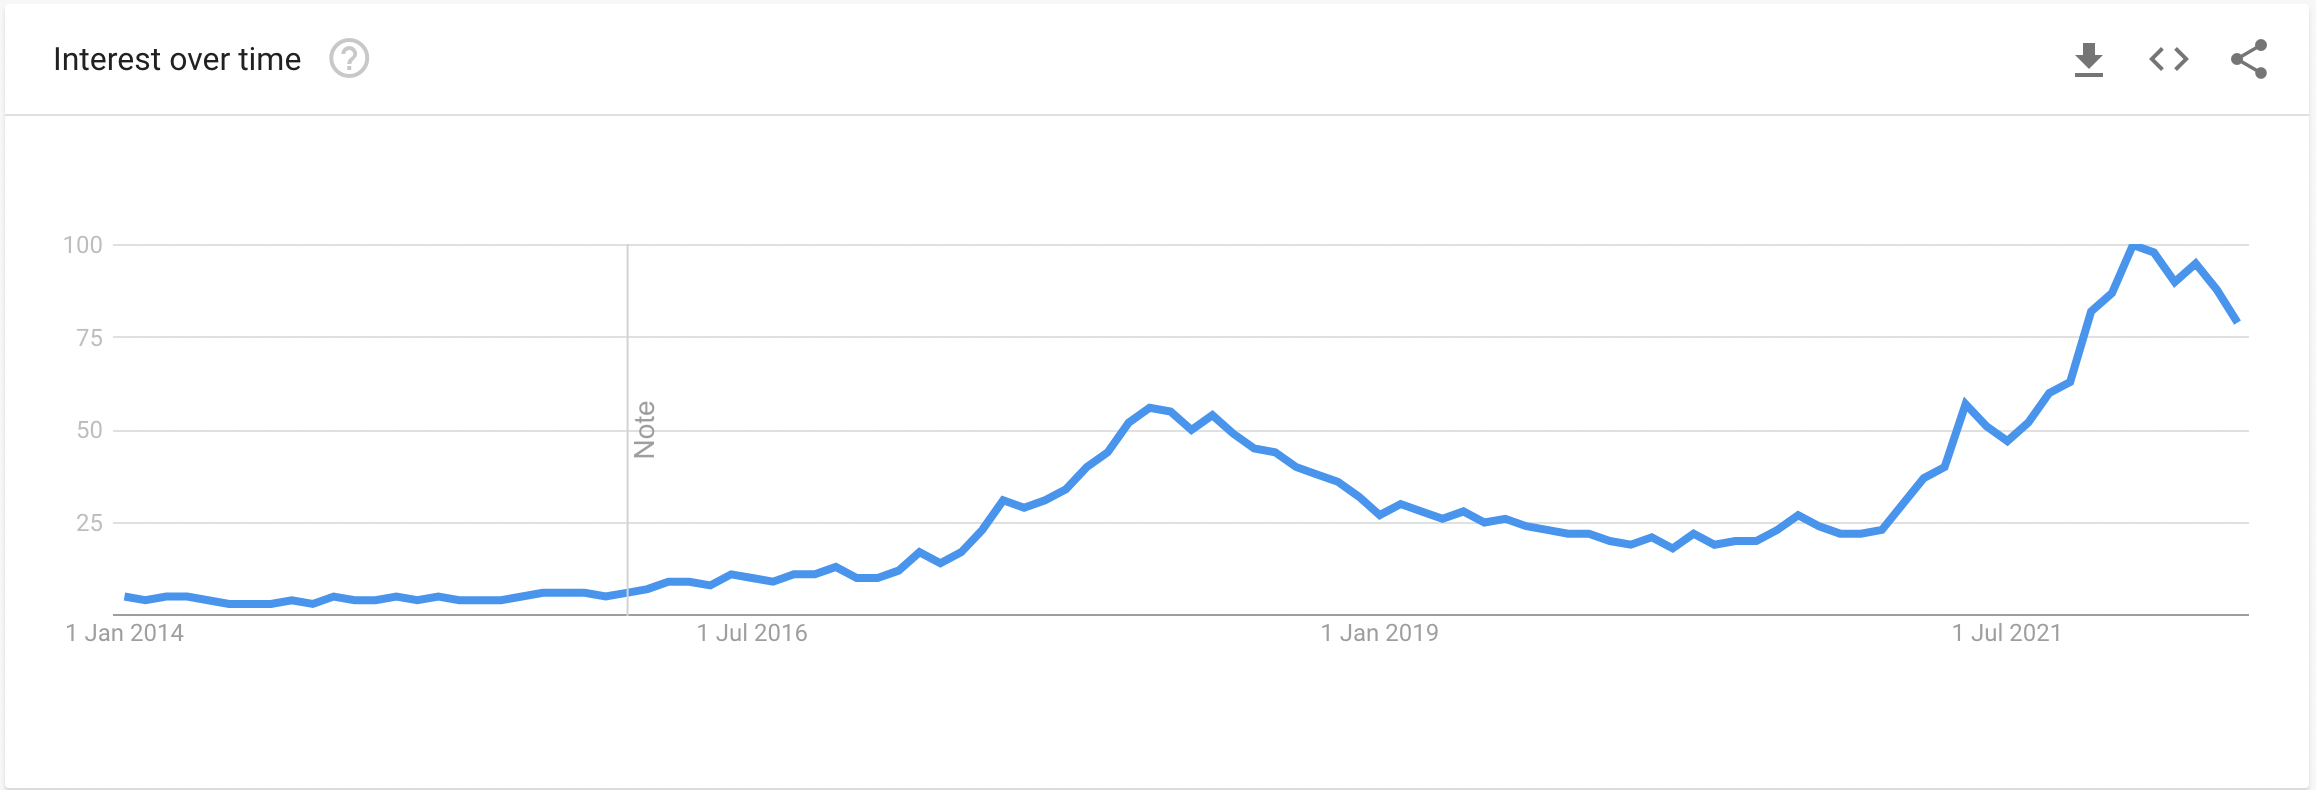
\includegraphics[width=15cm]{images/solidity_interest.png}
    \caption{Solidity interest from 1st of January, 2014, to 1st of June, 2022, according to Google web searches}
    \label{fig:solidity-interest}
\end{figure}

\begin{figure}
    \centering
    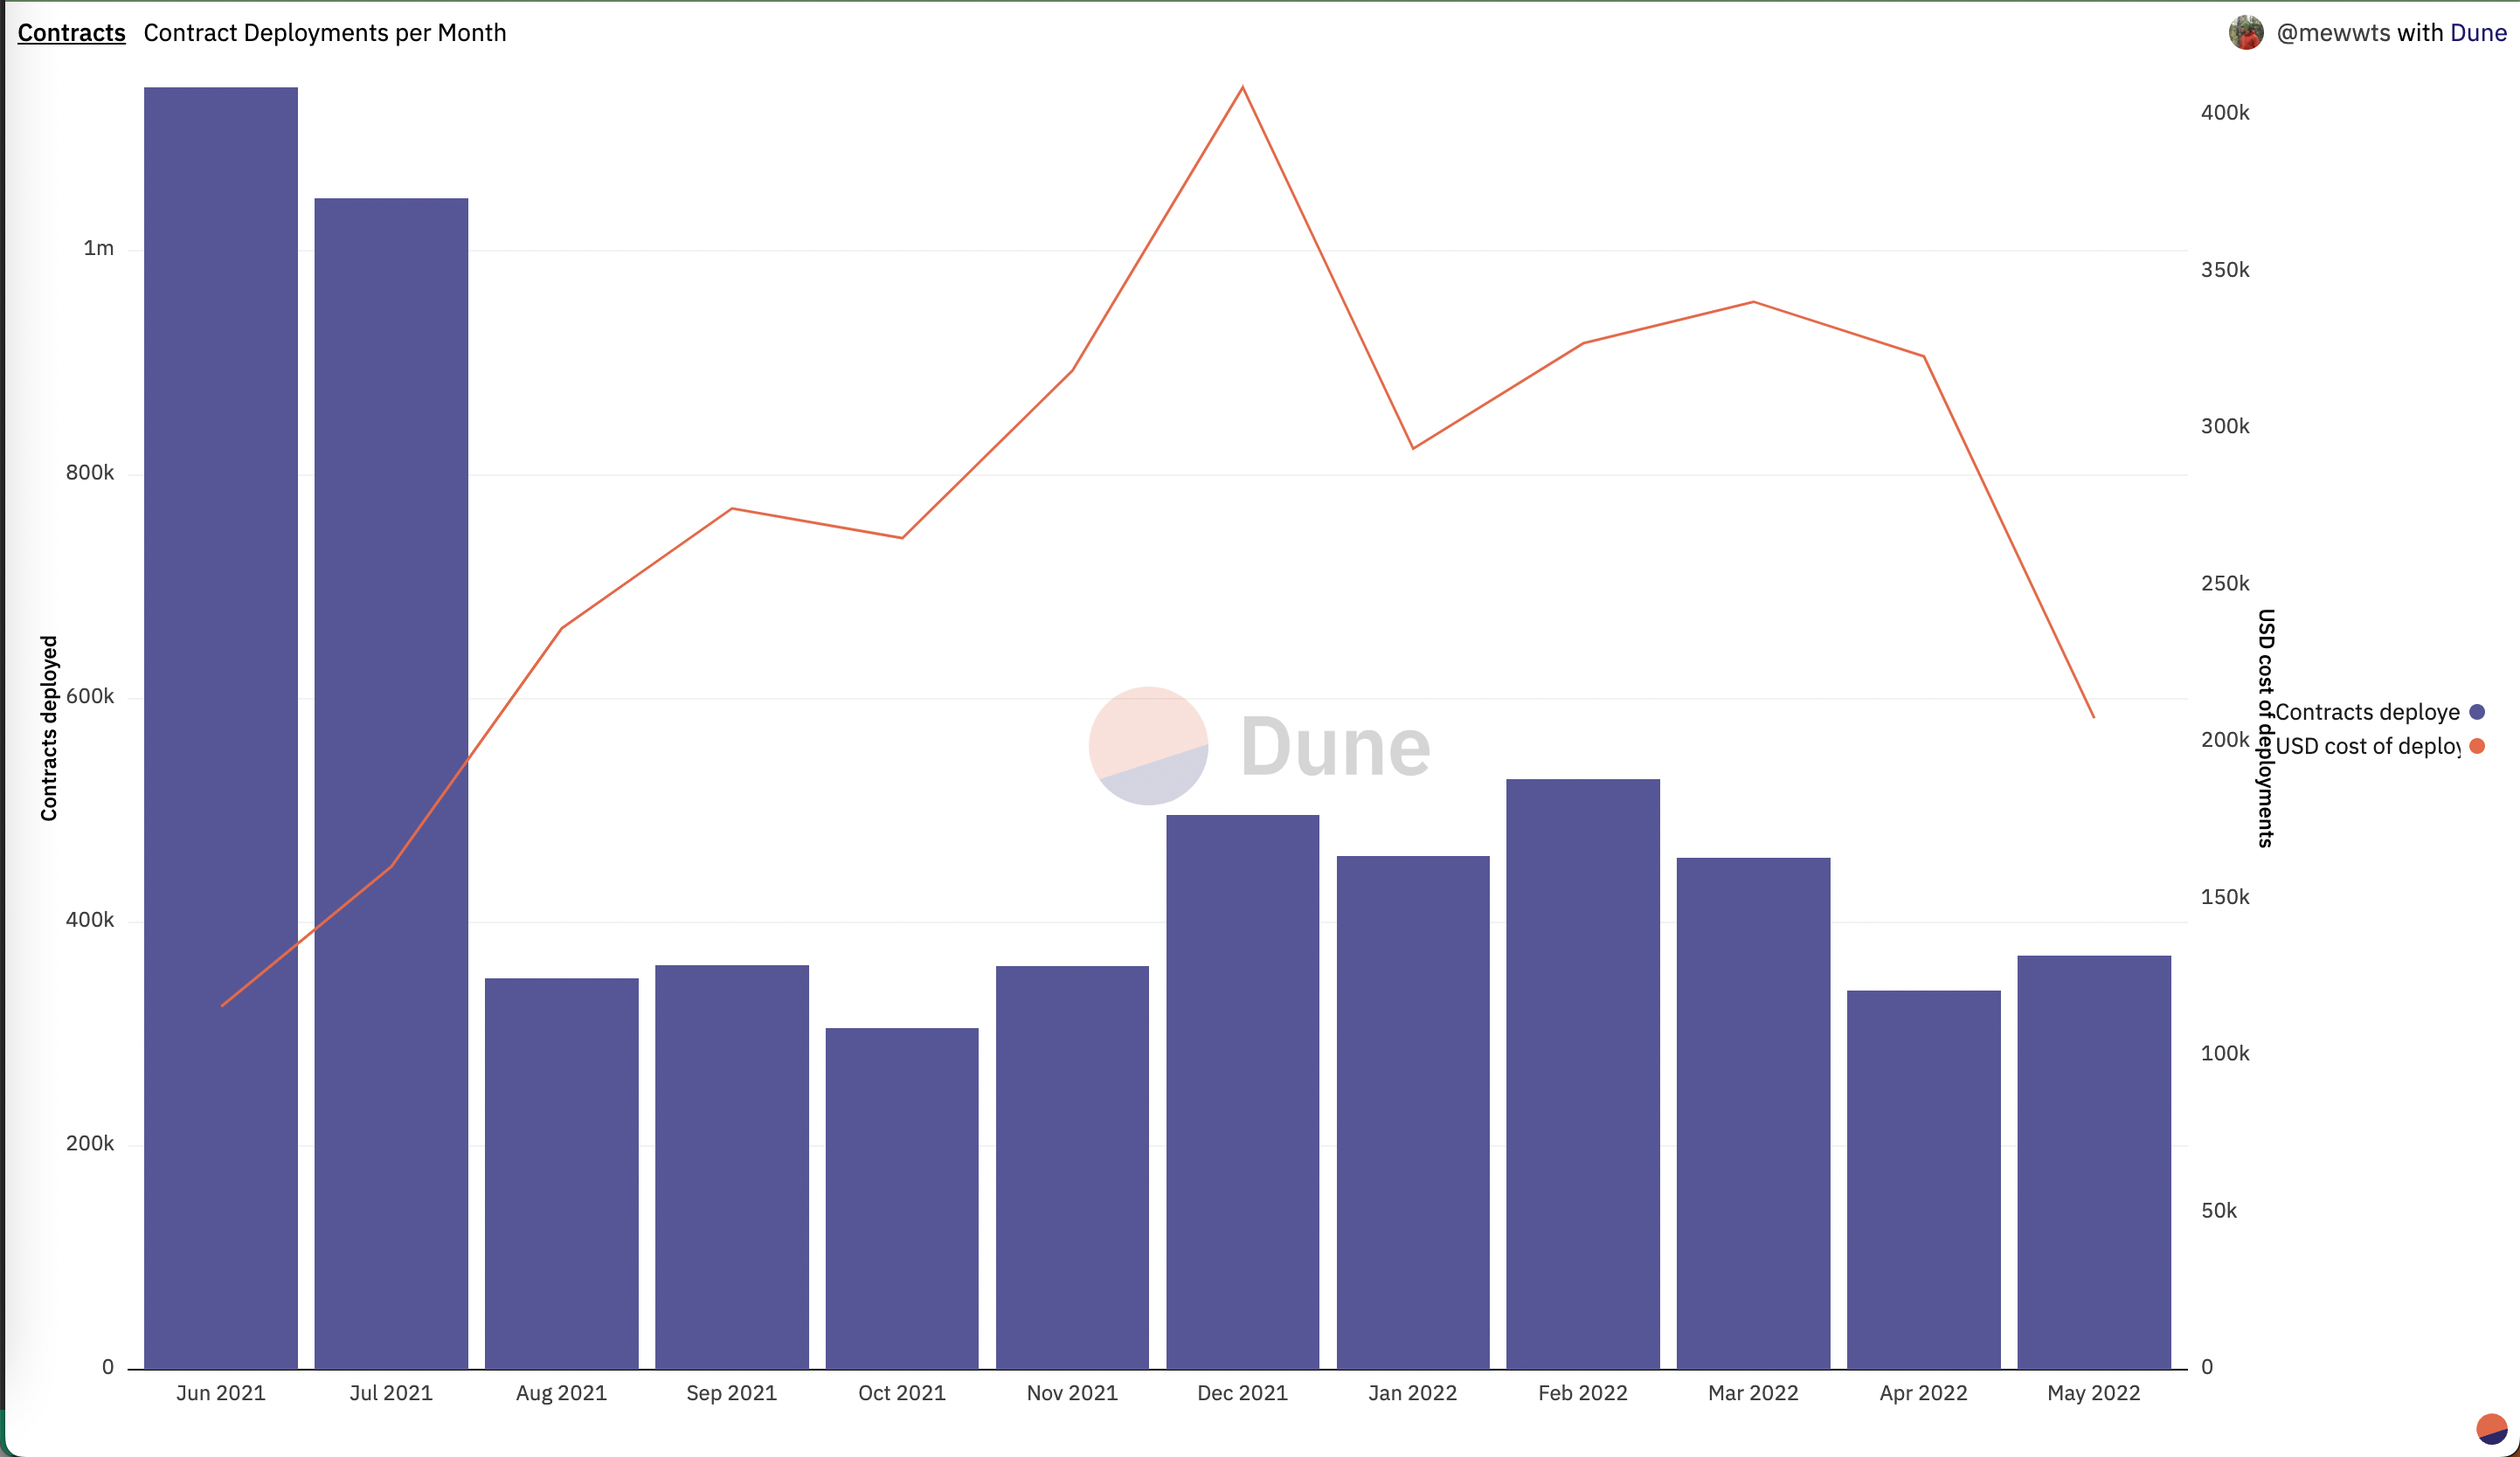
\includegraphics[width=15cm]{images/dune_analytics_2022.png}
    \caption{Contract deployment per month in the past year, according to Dune Analytics}
    \label{fig:dune-analytics-2022}
\end{figure}

\paragraph*{}
The main properties that interests this thesis are that this programming language is \textbf{statically typed} and is converted into bytecode to run inside the Ethereum Virtual Machine (EVM). Being statically typed helps the compiler with static analysis, making possible the development of an optimization suite that performs both common optimizations and particular optimizations for EVM.

\section{Solidity's Compiler and Optimizer}
\paragraph*{}
High level solidity code is sent to \lstinline[columns=fixed]{solc} binary, which stands for ``solidity compiler''. The user may or may not specify the usage of the optimizer with the \lstinline[columns=fixed]{--optimize} flag, which is enabled by default. Upon analyzing the compilation flow \ref*{fig:solc-compilation-flow}, we notice that there are some optional (yet recommended) steps to follow while compiling, which take advantage of Yul (intermediate code representation for Solidity) and Abstract Syntax Trees, the latter being built for both the initial Solidity code and for the Yul IR. If we choose to optimize the code through Yul, then the \lstinline[columns=fixed]{--via-ir} must be specified, which is also enabled by default.

\paragraph*{}
When optimizing through Yul, the compilation flow will actually use \textbf{two optimizers}: the "new" one (Yul optimizer) and the "legacy" one (EVM bytecode optimizer). The reasoning behind this is that bytecode optimization should be as simple and straightforward as possible, this also being an engineering decision made by Solidity's team that they explained in the Solidity Summit presentations, 2022. \lstinline[columns=fixed]{JUMP} instructions are especially tricky to handle while optimizing bytecode, making high level, semantic optimization (for example simplifying \lstinline[columns=fixed]{for} loops) more difficult.

\paragraph*{}
The advantage of having two optimizers is that it decouples work by a great deal. Low level assembly optimizations are done by the legacy optimizer \footnote{Future work might also consist in unifying EVM and LLVM, bringing all of the work and optimization done to LLVM on Solidity's ground as well.}, and more complex optimizations, that require techniques such as data flow analysis, are done directly on the Yul IR, which is later used to generate the efficient bytecode. This also helps to visually inspect the generated Yul IR and making sure that its output is the expected one. Specifically for the team, it means that it makes unit testing and development much easier.

\begin{figure}
    \centering
    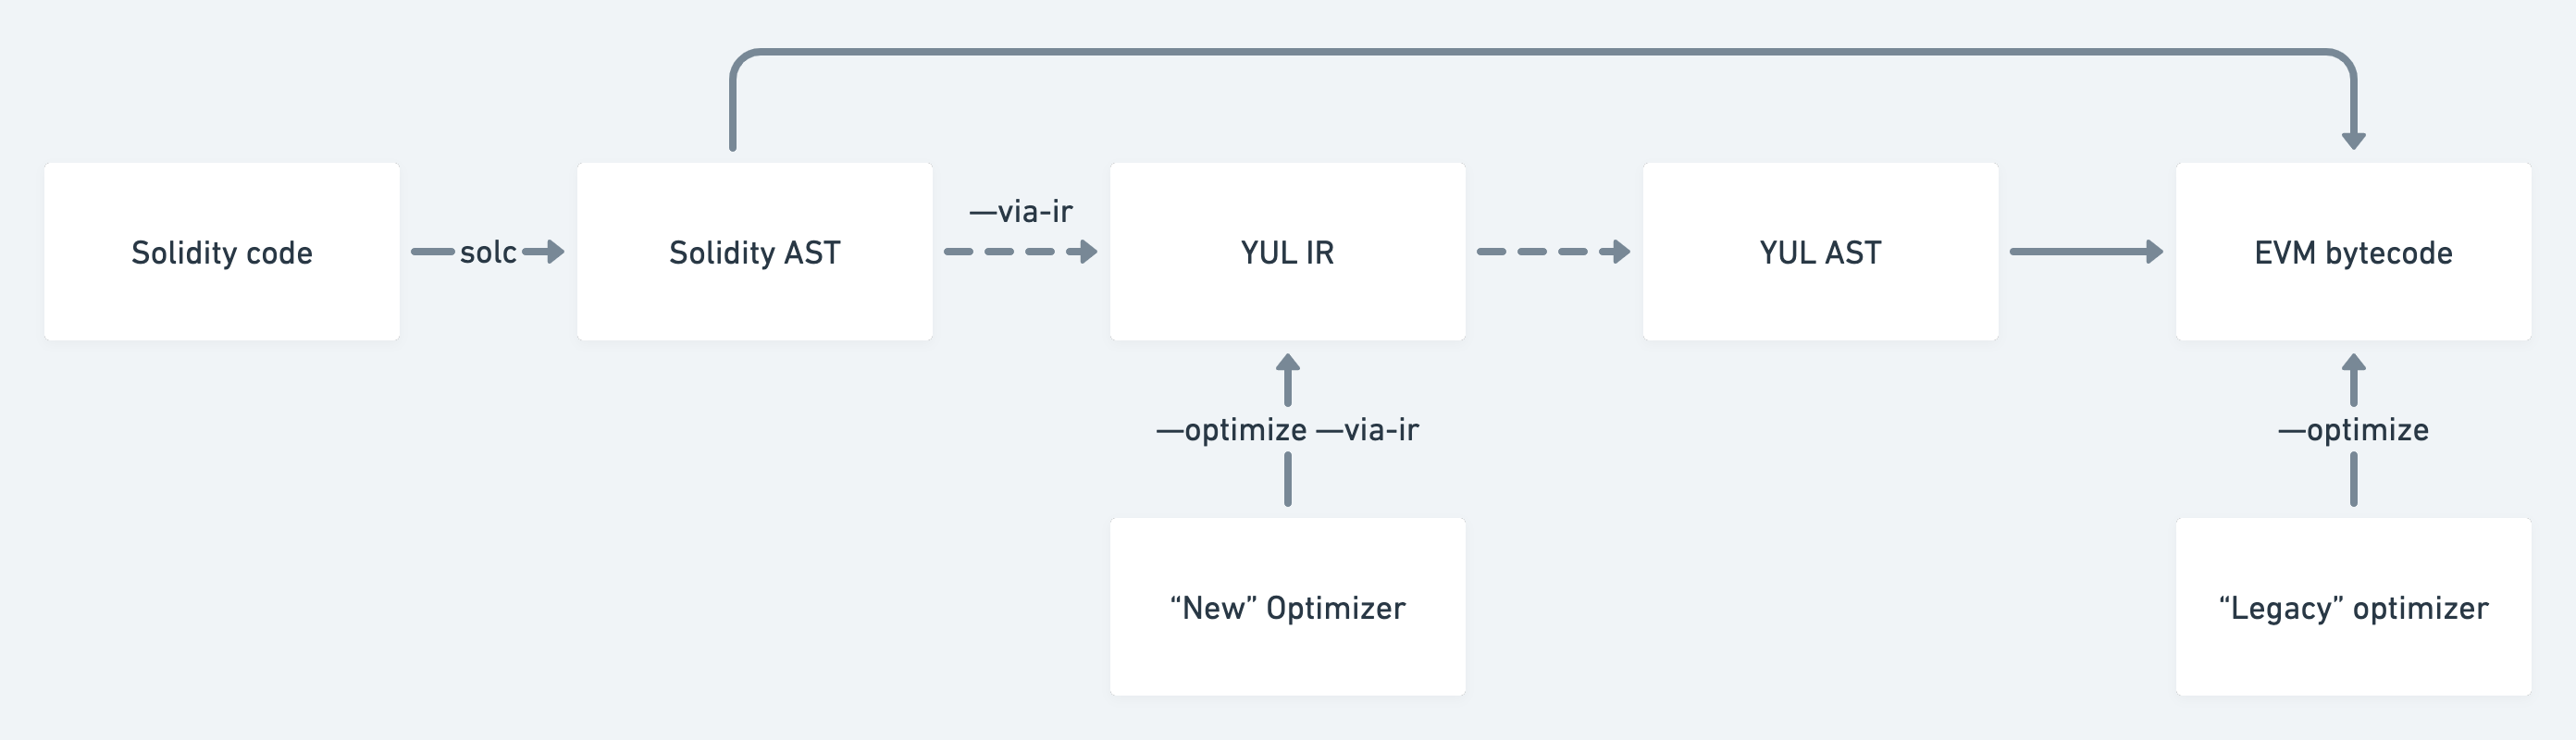
\includegraphics[width=15cm]{images/solc_flow.png}
    \caption{Solidity compilation flow}
    \label{fig:solc-compilation-flow}
\end{figure}

\section{Intermediate Representations}

\subsection*{Abstract Syntax Tree}
\paragraph*{}
\textbf{Abstract Syntax Trees (AST)} are often used to do a first analysis of the code instructions by walking the tree. This is often coupled with the Visitor Design Pattern, where the user implements what the \lstinline[columns=fixed]{visit} function should do for each type of node. They are often used in compilers to represent the structure of the code, to make isolated code changes and then re-generate code from the AST.

\paragraph*{}
Solidity uses ANTLR (ANother Tool for Language Recognition) to generate its AST. On Solidity's territory, ASTs appear in two phases. First, an AST is generated from the unaltered Solidity code, while another AST is later generated from the Yul IR code. The AST nodes provide sufficient granularity to make a structural analysis simple enough, thanks to recursively analysing the children node of a root.

\begin{figure}
    \centering
    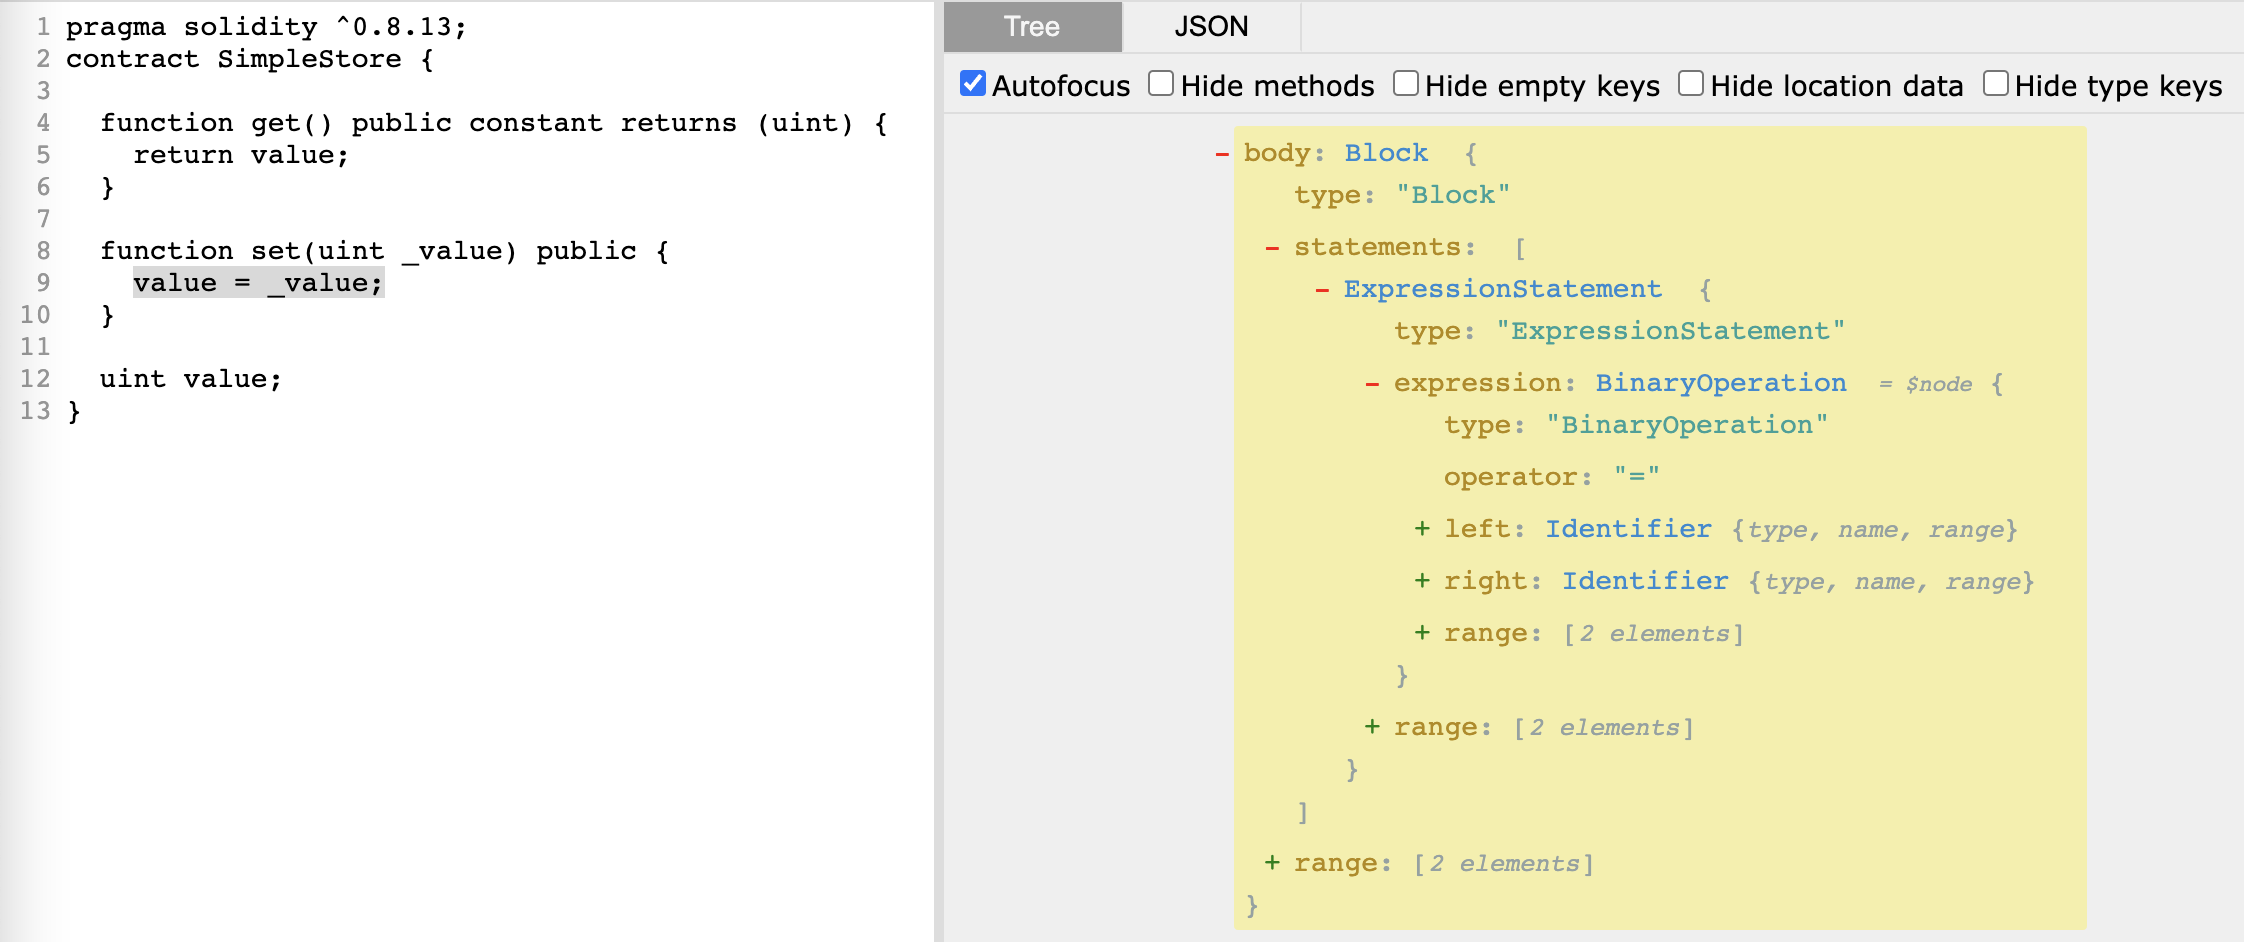
\includegraphics[width=15cm]{images/solidity_ast_example.png}
    \caption{Solidity AST Example. The body of the function is an AST node itself, in which the statements are other AST nodes. Generated using AST Explorer.}
    \label{fig:solidity-ast-example}
\end{figure}

\paragraph*{}
ASTs are very common in static analysis and are often times coupled with a grammar (or dialect) that enforces different node types and node structure in the tree. There are a variety of tools that use ASTs to do code analysis of their own.

% ASTs generated from Solidity code have been used by a variety of tools to inspect code, one of which is Solidity Instrumentation Framework (SIF) \ref{fig:sif-workflow}. The framework builds an internal representation (in C) of the AST nodes, bringing an additional set of features such as symbol renaming or function listing to the table. This works by exposing the \lstinline[columns=fixed]{visit} function to the user, each node being visited with the pattern implemented by the user.


\subsection*{Yul IR}
\paragraph*{}
\textbf{Yul}, former name Julia, is an intermediate representation for Solidity Code. It has been publicly announced as ``production ready'' in March, 2022, in version 0.8.13 of Solidity. Since then, the engineering team has been encouraging people to compile smart contracts via the usage of Yul, since the optimization focus has shifted on this pseudocode language.

\paragraph*{}
Yul was designed around four main principles, as described by its official documentation \cite{yul-description}: readability, easy manual inspection of control flow, simple and straightforward generation of bytecode from Yul and whole-program optimization. As compared to bytecode, this IR provides high-level syntax for instructions that introduce jump instructions (\lstinline[columns=fixed]{JUMP, JUMPDEST, JUMPI}), the reasoning behind this being that it makes analyzing data flow and control flow in the code much easier.

\begin{lstlisting}[caption={Example of Yul code which computes exponentiation recursively}]
{
    function power(base, exponent) -> result
    {
        switch exponent
        case 0 { result := 1 }
        case 1 { result := base }
        default
        {
            result := power(mul(base, base), div(exponent, 2))
            switch mod(exponent, 2)
                case 1 { result := mul(base, result) }
        }
    }
}
\end{lstlisting}

\paragraph*{}
This was designed as an actual programming language, making it possible to generate valid EVM bytecode from Yul code. Of course, it is not recommended to write smart contracts in Yul, but one can do so to get more familiar with the dialect. It also takes on the property of its "parent" code, and is also statically typed as Solidity. This further eases the static analysis done by the compiler.

\begin{figure}
    \centering
    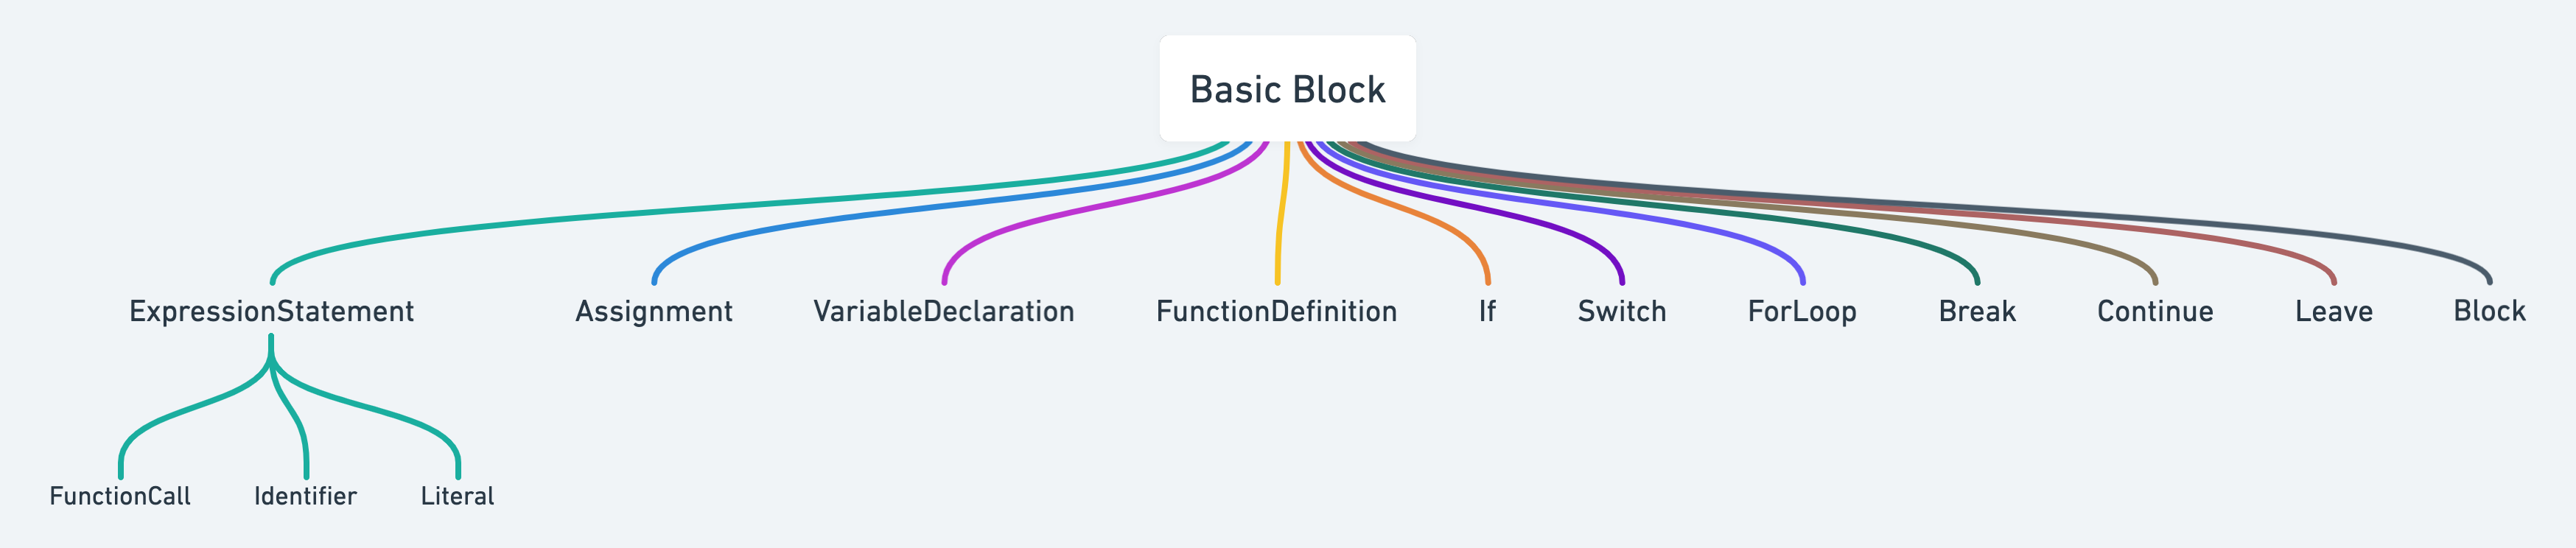
\includegraphics[width=\textwidth]{images/yul_ast_node_types.png}
    \caption{Node types in the YUL AST. Node properties vary depending on their nature.}
    \label{fig:yul-ast-node-types}
\end{figure}


\section{Other tools performing static analysis}
\paragraph*{}
The compiler has the option of outputting the Solidity AST in JSON format, which means that external tools can be built to alter the AST in any desired way. Since the compiler also supports receiving an AST as input, and generate bytecode from that one, that means that in theory one could build a better optimizer than the official one. While that hasn't happened yet, there are a few tools that perform code analysis of their own.

\subsection{Solidity Instrumentation Framework (SIF)}

Built by Chao Peng, Sefa Akca and Ajitha Rajan, from University of Edinburgh, SIF is a tool built in C that gravitates around the Visitor Design Pattern. The main objective is to build an internal C representation of Solidity code, through intermediary data structures, upon which SIF can orchestrate various optimizations / refactoring functions. As the authors describe it, it's a tool \cite[to easily and effectively understand, manipulate and analyse Solidity code]{sif}.

\begin{figure}
    \centering
    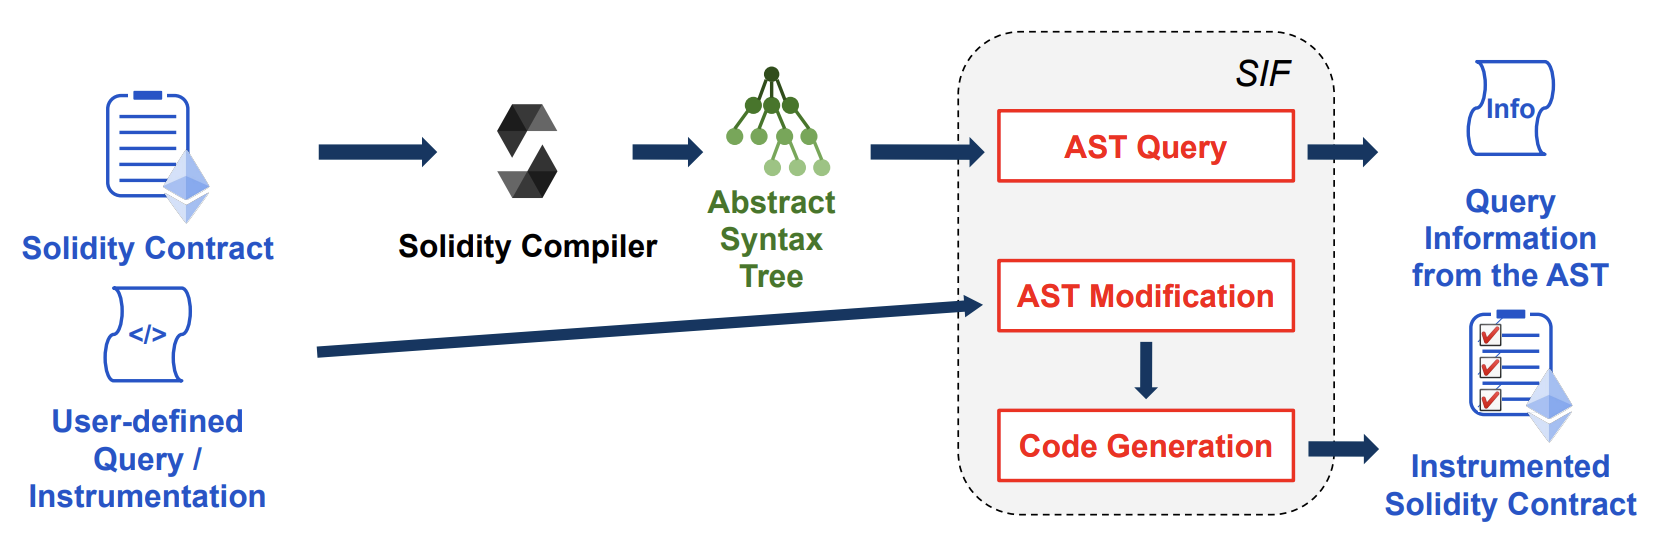
\includegraphics[width=15cm]{images/sif_workflow.png}
    \caption{SIF workflow, captured from SIF: A Framework for Solidity Contract Instrumentation and Analysis \cite{sif}}
    \label{fig:sif-workflow}
\end{figure}

The drawbacks that this toolkit currently has is that it's outdated and that it does not allow for external users to "plug-in" their own intermediate representations of Solidity code. It acts more as a middle-man, allowing users to implement, through the \emph{visit} method, specific optimization / refactoring items that run against isolated pieces of code. The tool does build a Control Flow Graph for the code, the one that this thesis will focus on, but it does not specifically use it for any kind of in-house optimization - it is just available to the user for usage. However, the completeness of the internal control flow graph is questionable.

\subsection{Slither}
\paragraph*{}
Slither is a more abstract, high level static analysis framework, which gives a broader overview over the internals of an Ethereum smart contract. Its main focus is centered around 4 areas: security (vulnerability detection), automated code optimization, code analysis and assisted code review, as described in Section 4.1 by the author Margherita Renieri \cite{slither}.

The tool takes advantage of the Abstract Syntax Tree (AST) built by the Solidity Compiler, then passes that through a series of optimization steps: Information Recovery, SlithIR Conversion and Code Analysis.

What's common in both of the tools we've seen is the usage of Abstract Syntax Trees and Control Flow Graphs, as well as building "proprietary" intermediate representation of the input code.

\begin{figure}
    \centering
    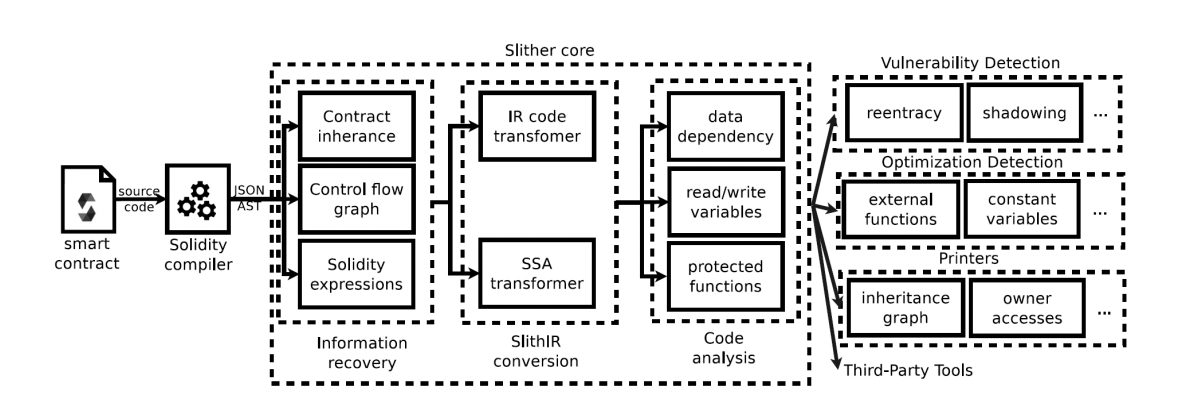
\includegraphics[width=15cm]{images/slither_architecture.png}
    \caption{Slither Architecture}
    \label{fig:slither-architecture}
\end{figure}

\subsection{Why focus on the official optimizer}
\paragraph*{}
The issue with such tools as SIF or Slither is that they get rapidly deprecated, since Solidity ground is so volatile, and they don't provide better optimization flows than Solidity's compiler does. Furthermore, integration is a bit more difficult, since it requires a separate optimization pipeline to be run through this intermediary tools, which just adds an additional burden to generating efficient bytecode.

What is certain is that the official compiler and optimizer will stay at the core of generating the Solidity bytecode. Therefore, any improvements to that will reflect itself in the next Solidity release - given it passes the team's rigurous reviews, of course. % Solidity, YUL IR, Compiler, Old vs new Optimizer
    \chapter{Contributions}

Solidity is a relatively new technology, when compared to already existing programming languages widely used in the market. As stated by the Solidity team itself, "the optimizer is under heavy development" \cite{solidity-optimizer}, which gives plenty of room for contributors to bring their own performance enhancements.

I plan on being one of those contributors, starting from the Solidity code and the AST built by the Solidity compiler itself. I will then evaluate the given inputs and focus on building a specific, low resolution Control Flow Graph, by which memory allocation and cpu cycles can be thoroughly inspected. This would allow for a technical deep dive into the insides of an Ethereum smart contract, which in return can provide useful insights to the user as to how the code can be optimized.

As compared to the other existing tools, this thesis will focus on the latest stable version of Solidity (0.8) and will be built around a set principles focused on scalable, maintainable code analysis tools. Security will also not be the main concern, as there is already plenty of interest in that area. % Static analysis, control flow graphs
    \chapter{YUL Optimizer Deep Dive}
\section{Optimization flow}
\paragraph*{}
As seen in the solidity compilation flow \ref{fig:solc-compilation-flow}, solidity optimizes its code via an \textbf{optimizer suite} which runs against the YUL IR. This consists of currently 32 documented steps \cite{solidity-yul-optimizer}, followed by a series of bytecode (opcode) optimizations which we will not focus on in this chapter. Some of the optimization steps are required to be run first, as they impose a specific structure to be further used and also make it safe to run arbitrary sequences of optimization steps \cite{solidity-yul-optimizer}, and are run in the following order:
\begin{enumerate}
    \item \textbf{Disambiguator}: returns a copy of the YUL AST where each variable has a unique identifier. Therefore, an AST walker can maintain a global state with regards to all of the identifiers in the code, even if we have variables with the same name in different parts of the program. This property is maintained by any subsequent step and there are no identical identifier names introduced while optimizing.
    \item \textbf{FunctionHoister}: moves all function definitions to the topmost block to enable isolated optimization of function definitions.
    \item \textbf{FunctionGrouper}: reorders code, such that the YUL code is of the form ${I \ F\ldots}$, where $I$ are instructions of the (possibly empty) entry block in the CFG and $F$ contain \textbf{un-nested} function definitions.
    \item \textbf{BlockFlattener} flattens nested blocks of code of form $\{\{ B \}\}$ to $\{ B \}$ if possible, i.e. if no interrupting control flows appear between the code blocks.
\end{enumerate}

% All components of the Yul-based optimizer module are explained below. The following transformation steps are the main components:

% SSA Transform

% Common Subexpression Eliminator

% Expression Simplifier

% Redundant Assign Eliminator

% Full Inliner


\paragraph*{}
Optimization makes a big difference. In code sample \ref{code:variable-declaration} we compute gas cost to re-declare a variable inside a for loop. When not optimized, the execution gast cost estimates for running \lstinline[language=Solidity]{declareVariableOutsideLoop} is $415250$ gas and \\ \lstinline[language=Solidity]{declareVariableInsideLoop} is $420223$ gas. This is expected, since the latter re-declares the same variable in every loop iteration.

\paragraph*{}
When optimized, however, gas usage is almost four times better, with \\ \lstinline[columns=fixed, language=Solidity]{declareVariableOutsideLoop} estimated to $119194$ gas and \lstinline[columns=fixed, language=Solidity]{declareVariableInsideLoop} to $119211$. An important note here is that the gas difference comes from the \textbf{function dispatch}, as described by Hari Mulackal \cite{hari-gas-dispatch}, i.e. the order of the functions in a contract introduce a small overhead. Specifically for this case, the optimization comes from the LoopInvariantCodeMotion step, which moves declarations (not assignments) outside the for loop.


\label{code:variable-declaration}
\begin{lstlisting}[language=Solidity, caption=Code example of bad variable declaration inside a for loop]
    // SPDX-License-Identifier: MIT
    pragma solidity ^0.8.14;

    contract VariableLoop {
        function declareVariableInsideLoop() public pure {
            for (uint i = 1; i <= 1000; i++) {
                uint x = i * i;
            }
        }

        function declareVariableOutsideLoop() public pure {
            uint x;
            for (uint i = 1; i <= 1000; i++) {
                x = i * i;
            }
        }
    }
\end{lstlisting}

\paragraph*{}
\textbf{Order matters} when running the optimization steps. In version 0.8.14, the default order \footnote{Optimization order is given by the step abbreviations, where each letter corresponds to an optimization phase. The mapping is described in the \href{https://docs.soliditylang.org/en/v0.8.14/yul.html}{Optimization Step Sequence section in the documentation}.} of the suite is

\begin{lstlisting}
    dhfoDgvulfnTUtnIf[xa[r]EscLMcCTUtTOntnfDIulLculVcul [j]Tpeulxa[rul]xa[r]cLgvifCTUca[r]LSsTFOtfDnca[r]Iulc]jmul[jul] VcTOcul jmul
\end{lstlisting}

In the above order, the optimizers between brackets \cite[will be applied multiple times in a loop until the Yul code remains unchanged or until the maximum number of rounds (currently 12)]{solidity-yul-optimizer}. We can immediately see that some of the optimizers are run more than once, the reasoning being that each optimizer may change the YUL IR, therefore giving new optimization opportunities to other optimizer. This is the case for UnusedAssignEliminator (r abbreviation) and UnusedPruner (u abbreviation). For example, let's optimize the following code in 2 rounds, first applying UnusedPruner and then UnusedAssignEliminator, then applying UnusedAssignEliminator and then UnusedPruner \footnote{The corresponding commands are \lstinline[columns=fixed]{solc --optimize --ir-optimized --via-ir --yul-optimizations 'ur' termination.sol} and \lstinline[columns=fixed]{solc --optimize --ir-optimized --via-ir --yul-optimizations 'ru' termination.sol}}:


\label{code:solidity-redundant-assignment}
\begin{lstlisting}[language=Solidity, caption=Example of a smart contract with a redundant assignment and variable declaration]
    // SPDX-License-Identifier: MIT
    pragma solidity ^0.8.14;

    contract Termination {
        uint persistent_var;
        event FunctionCalled(string f);

        function assignBeforeTermination() public {
            emit FunctionCalled("assignBeforeTermination");
            uint balance;
            balance = 7919;
            return;
        }
    }
\end{lstlisting}


\begin{figure}
    \centering
    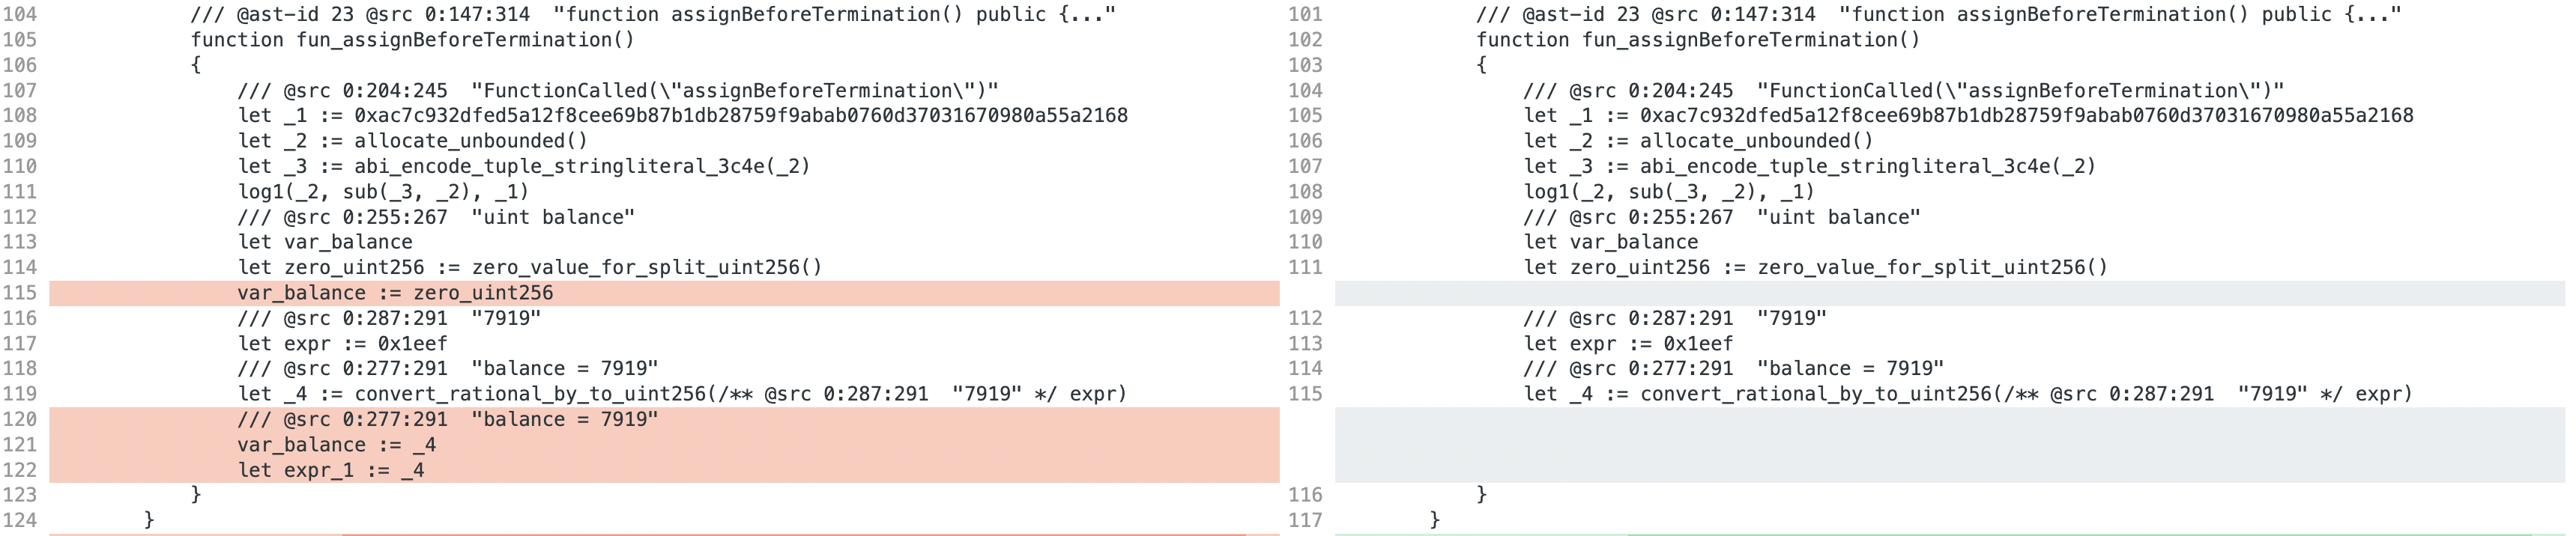
\includegraphics[width=\textwidth]{images/optimization_order_ur.png}
    \caption{Unoptimized vs. optimized YUL IR for Solidity code \ref{code:solidity-redundant-assignment}, order of optimizers: UnusedPruner then UnusedAssignEliminator}
    \label{fig:optimization-order-ur}
\end{figure}

\begin{figure}
    \centering
    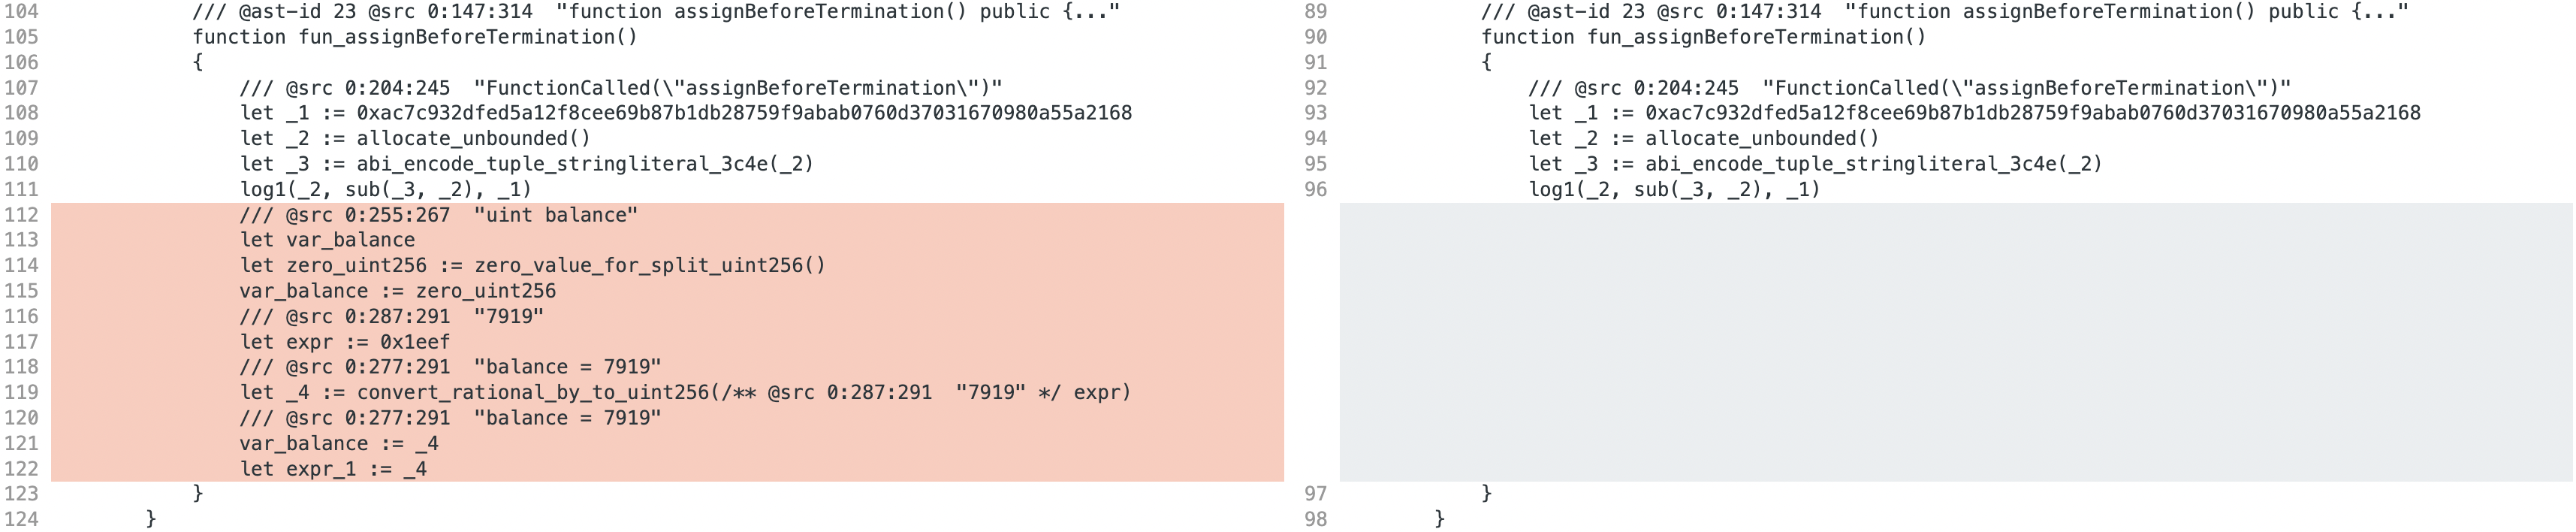
\includegraphics[width=\textwidth]{images/optimization_order_ru.png}
    \caption{Unoptimized vs. optimized YUL IR for Solidity code \ref{code:solidity-redundant-assignment}, order of optimizers: UnusedAssignEliminator then UnusedPruner}
    \label{fig:optimization-order-ru}
\end{figure}


\paragraph*{}
In the above figures \ref{fig:optimization-order-ru} \ref{fig:optimization-order-ur}, we have the same unoptimized YUL IR in the left-hand side, with the optimized YUL code on the right. Upon applying UnusedPruner, this step will look to remove any variable declarations that are not used. When applied first, it correctly identifies \lstinline[columns=fixed]{let expr_1 := _4} as a redundant variable declaration and it removes it. Afterwards, UnusedAssignEliminator runs and it finds \lstinline[columns=fixed]{var_balance := zero_uint256} and \lstinline[columns=fixed]{var_balance := _4} as redundant assignments and removes those as well. However, we can still notice some left-over assignments and variable declarations.

\paragraph*{}
If, however, UnusedAssignEliminator is run first, it removes the same assignments (\lstinline[columns=fixed]{var_balance := zero_uint256} and \lstinline[columns=fixed]{var_balance := _4}), but then gives more room for UnusedPruner to act. Therefore, all of the variable declarations get removed, since their values are not used and they are redundant.

\paragraph*{}
While this is a proof-of-concept example, optimizer steps frequently generate intermediary data objects (such as the SSATransform) to make local optimizations safe and possible (remember that corectness comes before optimization). Hence why these two optimizers are simple, yet effective.

\section{UnusedPruner. UnusedAssignEliminator.}
\paragraph*{}
A very effective way of reducing gas usage is by removing any kind of redundant variable assignments or variable declarations, since it implies executing less instructions. This can be applied as both a local optimization and as a global optimization. In case we locally prune variable declarations, we must ensure that other control flows do not have references to the the left-hand side of the assignment. For example, considering \ref*{code:assignment-sample}, we can see that the assignment at line 3 can be removed, since \lstinline[columns=fixed]{a} is immediately re-assigned. However, even though \lstinline[columns=fixed]{a} gets re-assigned at line 10, we cannot remove assignment at line 4, because there is another control flow that uses the latter assignment, in the \lstinline[columns=fixed]{if} statement. 

\label{code:assignment-sample}
\begin{lstlisting}[caption=YUL IR code sample for variable assignments. Both variables a and b are used in a different control flow.]
{
    let a
    a := 1
    a := 2
    b := 2
    if calldataload(0)
    {
        b := mload(a)
    }
    a := b
}
\end{lstlisting}

\subsection{Variable states in UnusedAssignEliminator}
\paragraph*{}
UnusedAssignEliminator acts in two phases: one to collect information and one to prune redundant assignments. While doing data flow analysis, it assigns different states to the identifiers \footnote{This optimizer only treats assignment where the left-hand side is a single identifier (variable)}: \textbf{undecided, used and unused}. It does so by acting as an YUL AST walker and visiting each VariableAssignment node. On the second pass, any assignment expression that is in the ``undecided'' state will be marked as ``unused'' and will be pruned from the AST, therefore from the final YUL IR code.

\paragraph*{}
An assignment \lstinline[columns=fixed]{a := b} will be marked as ``used'' only if there exists another expression $E$ within the same basic block $B$ or within a basic block $B'$ such that we have a path in the CFG from $B$ to $B'$, where $E$ contains \lstinline[columns=fixed]{a} on the right-hand side. Similarly, if such an expression $E$ does not exist, then the assignment can be marked as ``unused''.


\section{Handling termination flows}
\paragraph*{}
While getting acquainted with the compiler, several experiments have pointed out that the compiler does not treat all of the edge cases with regards to redundant assignments, especially when \textbf{termination flows} appear within basic blocks. YUL IR uses the EVM dialect where termination flows are given by the \lstinline[columns=fixed]{return}, \lstinline[columns=fixed]{revert}, \lstinline[columns=fixed]{selfdestruct} and \lstinline[columns=fixed]{invalid} instructions \footnote{It suffices to focus on the YUL IR instructions, since the optimization flow does not work with Solidity code directly.}. To understand the examples, we must note the different control flows that are present in the CFG for the YUL AST: FlowOut, Break, Continue, Terminate and Leave.

\begin{figure}
    \centering
    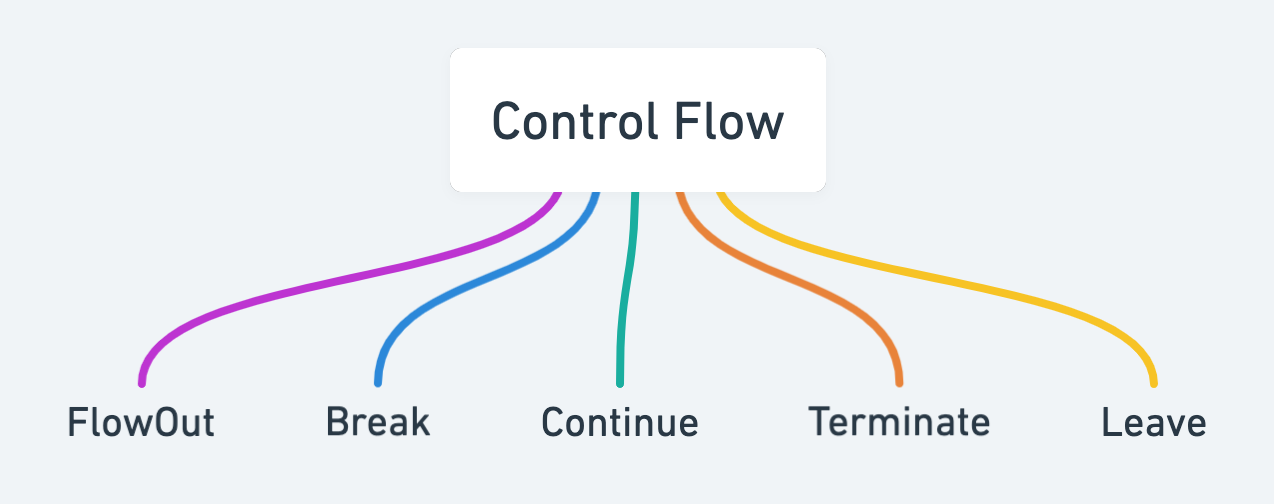
\includegraphics[width=10cm]{images/cfg_control_flow_types.png}
    \caption{Control flow types in YUL IR}
    \label{fig:cfg-control-flow-types}
\end{figure}

\paragraph*{}
All of the above except FlowOut are applied to simple, one-line statements. FlowOut is the most complex one and it embeds the normal execution of the program, as well as the terminal execution of a program. It is applied ``by default`` to \lstinline[columns=fixed]{for} loops \footnote{In YUL IR, \lstinline[columns=fixed]{while} loops get converted to \lstinline[columns=fixed]{for} loops}, \lstinline[columns=fixed]{if} statements, \lstinline[columns=fixed]{switch} statements and functions that can revert, stop or exit normally upon calling them.

\paragraph*{}
A successful attempt to ``fool'' the compiler was done by introducing a Terminate control flow after a redundant assign eliminator. The code sample is as follows:

\label{code:unused-assign-eliminator-handle-termination-flow}
\begin{lstlisting}[caption=YUL IR code sample for variable assignments. Both variables a and b are used in a different control flow.]
    // SPDX-License-Identifier: MIT
    pragma solidity ^0.8.14;
    
    contract Termination {
        uint persistent_var;
        event FunctionCalled(string f);
        event BalanceIsEmpty();
    
        function assignBeforeTermination(uint x) public {
            emit FunctionCalled("assignBeforeTermination");
            uint balance;
            
            if (f1(x) == true) {
                balance = 10007;
                return;
            }
    
            if (balance == 0) {
                emit BalanceIsEmpty();
            }
            return;
        }
    
        function f1(uint x) public pure returns (bool) {
            return x > 10;
        }
    }    
\end{lstlisting}

The introduced termination flow is at line 15, right after the assignment to variable \lstinline[columns=fixed]{balance}, which is then referenced inside the second \lstinline[columns=fixed]{if} condition. The usage of \lstinline[columns=fixed]{f1} functions is necessary to make it impossible for the compiler to compute the \lstinline[columns=fixed]{if} condition's value at compile time, i.e. introduce a \textbf{non-deterministic} flow. The compiler seens \lstinline[columns=fixed]{balance} as referenced in a different control flow, therefore it will not remove assignment at line 14. We can easily see, however, that if the condition \lstinline[columns=fixed]{f1(x) == true} does not stand, then the second if will always evaluate to true, hence why the StructuralSimplifier optimizer could be used to simplify things further and entirely remove the second if condition, since it will always evaluate be true if the termination flow is not executed.


\begin{figure}
    \centering
    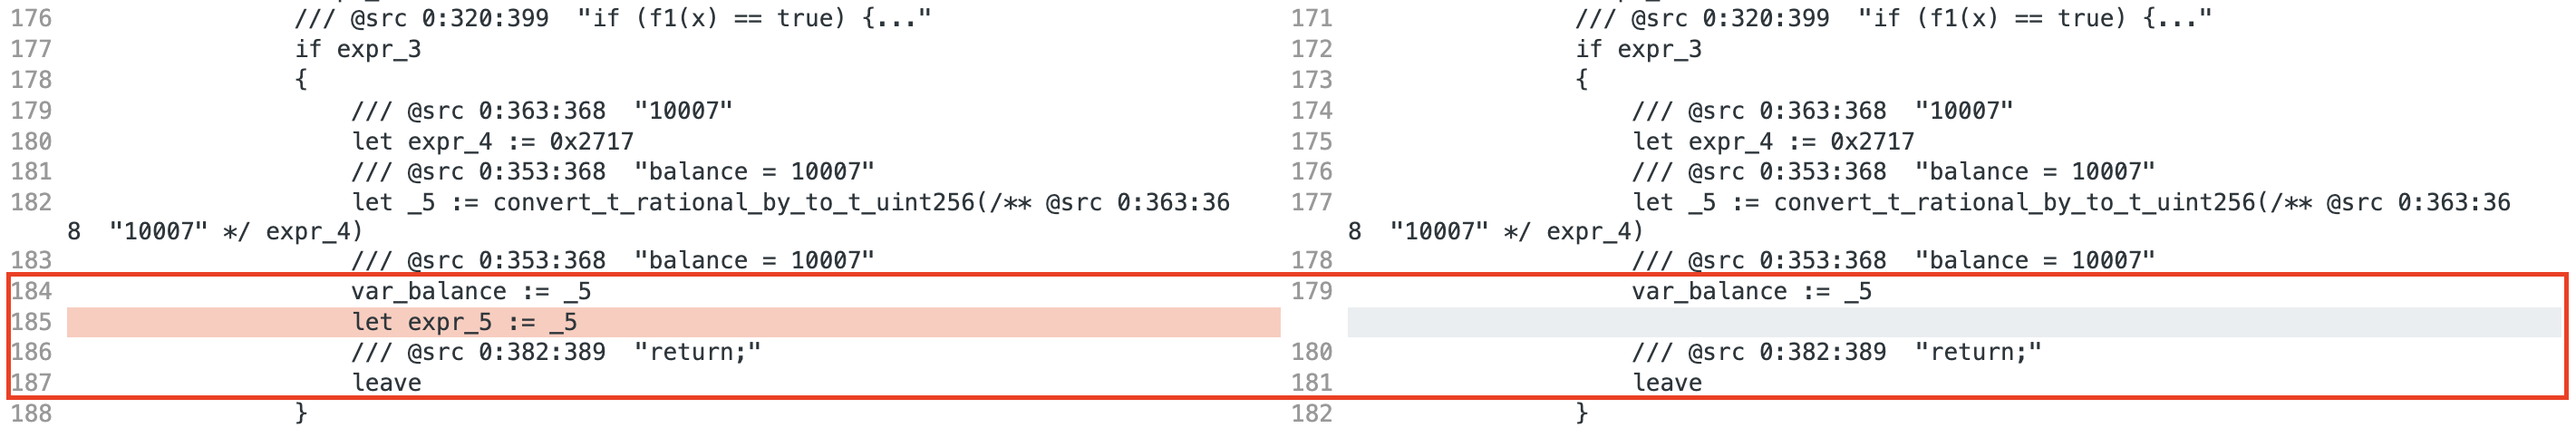
\includegraphics[width=\textwidth]{images/unused_assign_eliminator_termination2.png}
    \caption{Optimized YUL IR using UnusedAssignEliminator then UnusedPruner. UnusedAssignEliminator does not handle termination flows while pruning}
    \label{fig:unused-assign-eliminator-termination2}
\end{figure}

\paragraph*{}
To handle this edge case, we can simplify the problem of determining wether a basic block contains a termination flow or not. Figure \ref*{fig:basic-block-termination-ast-example} shows how a \lstinline[columns=fixed]{leave} statement could be following by valid YUL IR statements (i.e. dead Solidity code after a \lstinline[columns=fixed]{return} instruction). We use the DeadCodeEliminator step for this case to ensure that there are no instructions following an instruction that terminates the execution.

\begin{figure}
    \centering
    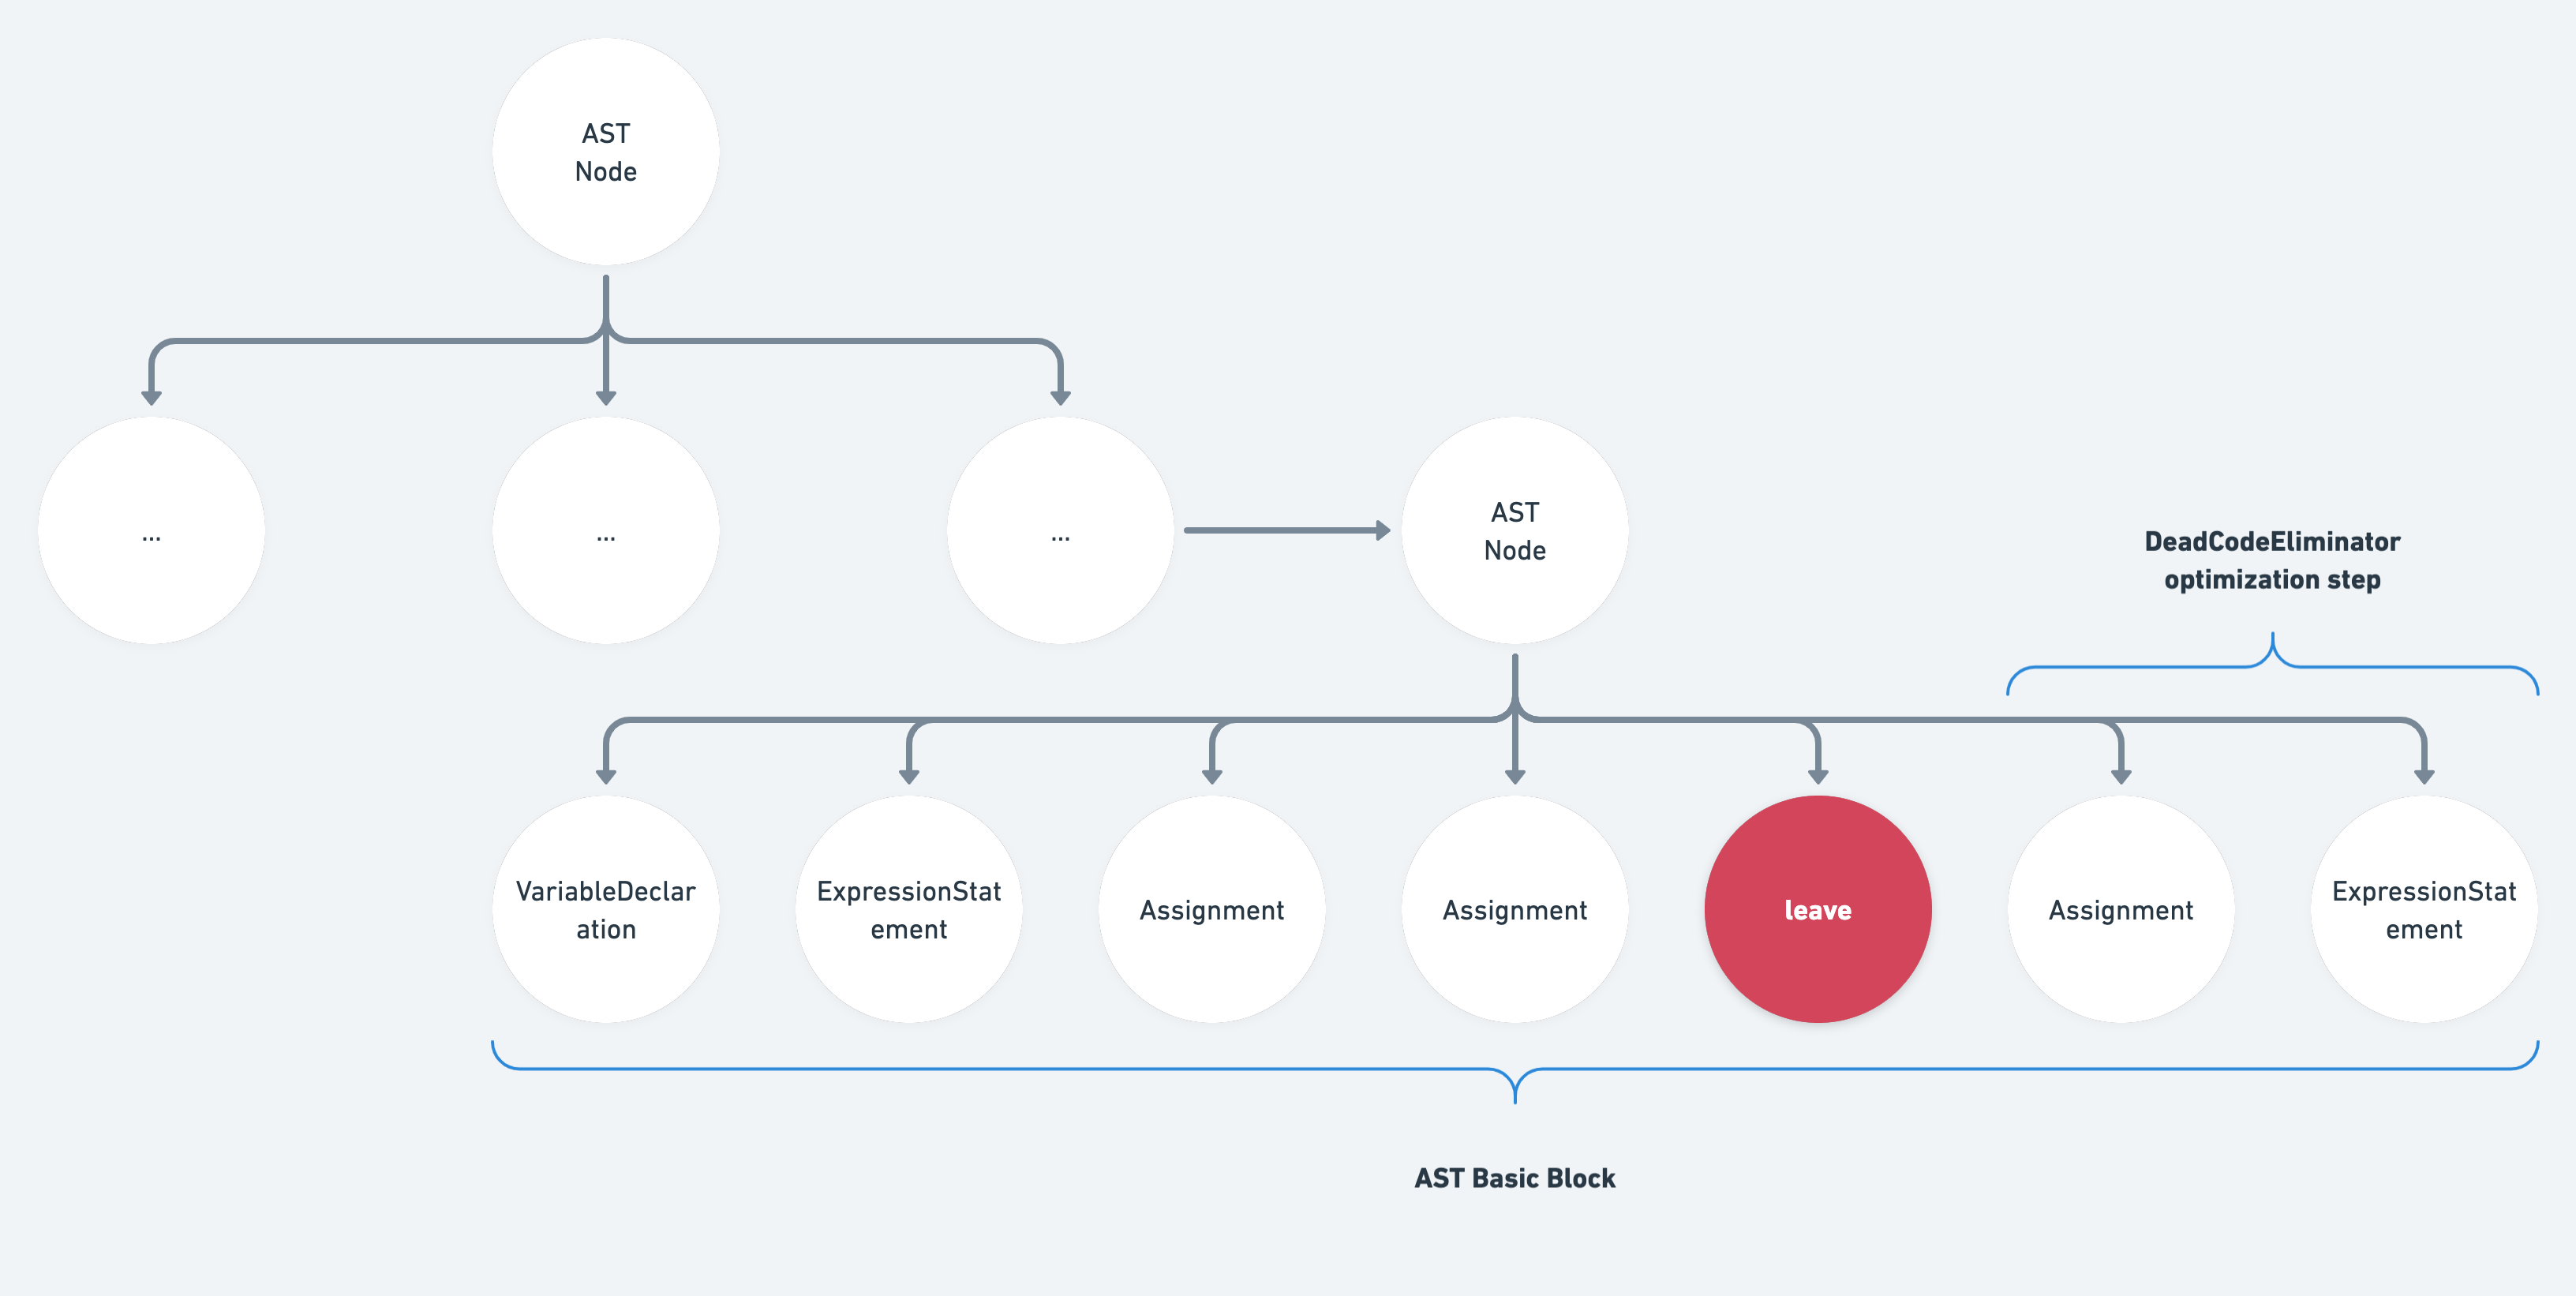
\includegraphics[width=\textwidth]{images/basic_block_termination_ast_example.png}
    \caption{Example of termination flow inside a YUL AST's basic block node. DeadCodeEliminator is used to prune unreachable code}
    \label{fig:basic-block-termination-ast-example}
\end{figure}

\paragraph*{}
With this simplification in mind, the edge case can be handled by enhancing the \\ \lstinline[columns=fixed]{UnusedAssignEliminator.visit} function for Basic Blocks in the YUL AST. That is, when visiting the block, we make a copy of the current recorded assignments (outside of the current basic block) such that after visiting we can compute the new assignments - this includes variable declarations. If basic block $B$'s body trailing statement induces a termination flow, then we can safely remove all of the new assignments made in that block, even if they are referenced in another block of the CFG.

\paragraph*{}
Some special cases must be considered however, such as \textbf{state variables} which are persistent within the contract. These are defined in Solidity as members of the smart contract. Obviously, any assignment to such a persistent variable $p$ \textbf{should not} be removed, regardless of the control flows that follows it. The only case in which we can safely remove them is if they consist unreachable code, which the DeadCodeEliminator will handle. We therefore restrict the behaviour of the above enhancement to only local basic block variables or to the inputs of the basic block \footnote{This is actually easy to do because persistent variables are kept in memory. Their values are updated via function calls, which are not recognized by the AST walker as variable assignments / declarations.}.

\paragraph*{}
The Solidity compiler reports that the estimated gas usage for the contract construction for code sample \ref*{code:unused-assign-eliminator-handle-termination-flow} went down from $67723$ to $65723$, a saving of $2000$ gas. Also, the execution of the \lstinline[columns=fixed]{assignBeforeTermination} function went down from $2585$ to $2565$, which is $20$ gas less. The result of the enhancement can be seen in figure \ref{fig:unused-assign-eliminator-handle-termination-flow} where the full optimizer suite was ran against the same code sample, with and without the above enhancement. This also enabled StructuralSimplifier to simplify code further, completely removing the second \lstinline[columns=fixed]{if} condition and un-nesting the emitting of the \lstinline[columns=fixed]{BalanceIsEmpty} event.


\begin{figure}
    \centering
    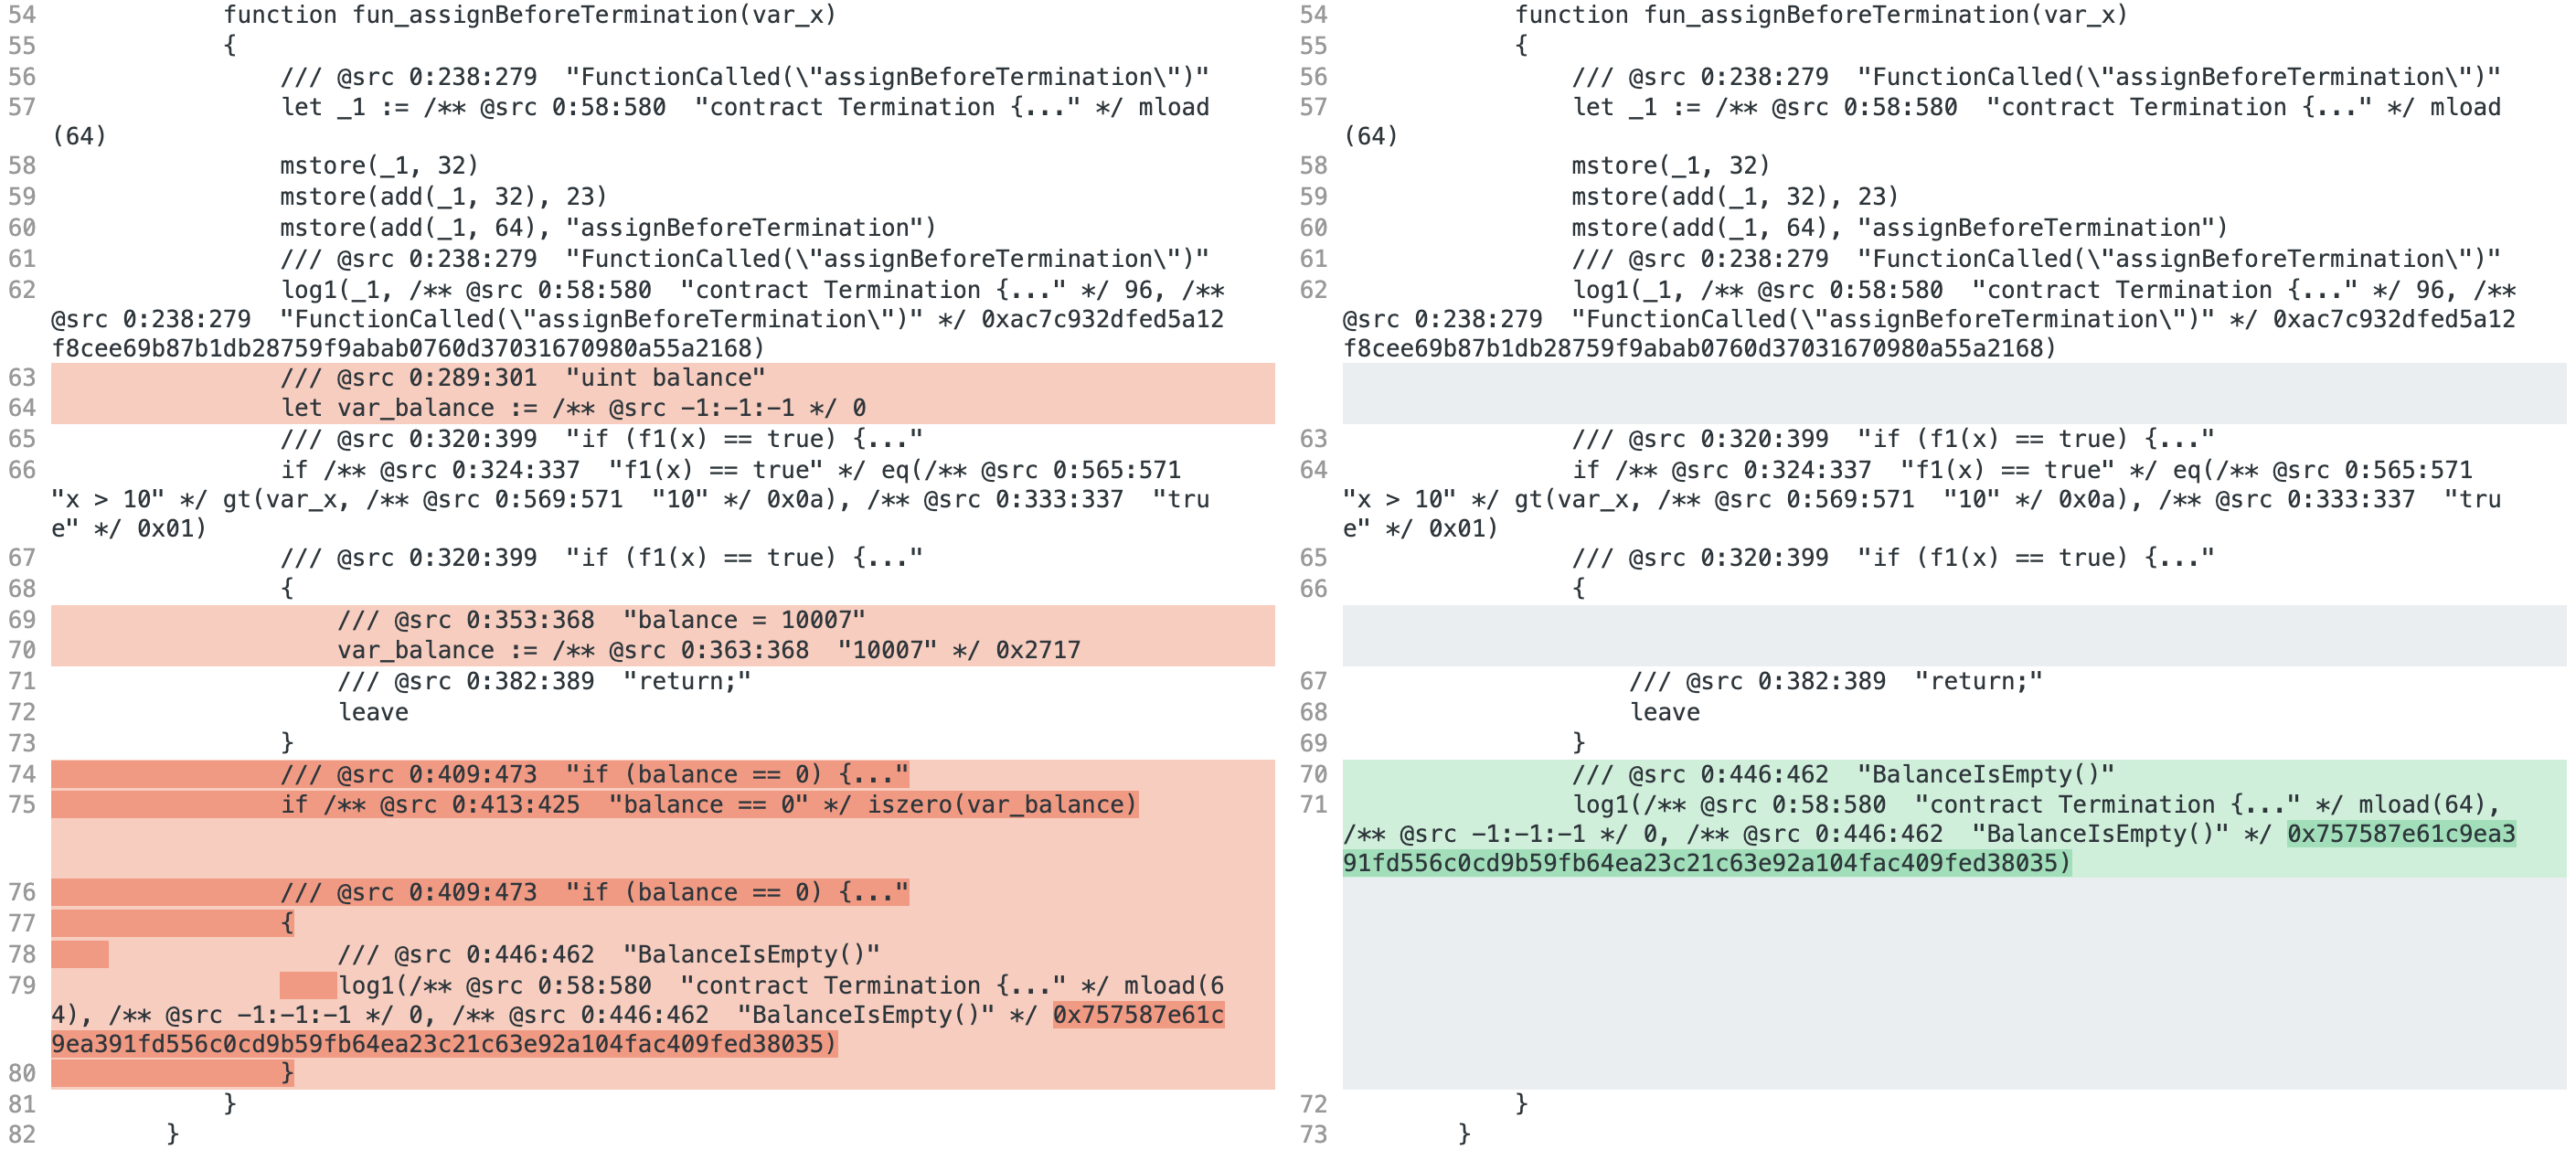
\includegraphics[width=\textwidth]{images/unused_assign_eliminator_handle_termination_flow.png}
    \caption{Full optimizer suite ran against code sample \ref{code:unused-assign-eliminator-handle-termination-flow}. The right hand side YUL IR handles termination flows within basic blocks for variable assignments and declarations.}
    \label{fig:unused-assign-eliminator-handle-termination-flow}
\end{figure}


\section{Pruning redundant termination flows}
\paragraph*{}
As stated in the previous chapter, running an optimization step $X$ may give more opportunities to optimization step $Y$ to further enhance the YUL IR (therefore the resulted bytecode). This was the case for the above enhancement, where experiments pointed out that if a basic block contains a trailing \lstinline[columns=fixed]{if} statement, then pruning code inside the \lstinline[columns=fixed]{if}'s body may result in a single trailing, redundant \lstinline[columns=fixed]{leave} instruction within the body. The expected basic block pattern for this case is
\begin{lstlisting}
    { ... if (C) { leave } }
\end{lstlisting}
after the removal of redundant code has been done.

\label{structural-simplifier-cascading-example}
\paragraph*{}
A good solution for this edge case was changing how the StructuralSimplifier works and make it look for \lstinline[columns=fixed]{leave} statements within an \lstinline[columns=fixed]{if}'s body. If that's the case, then the \lstinline[columns=fixed]{leave} statement is simply removed. This enabled for cascading enhancements, and the StructuralSimplifier will further completely remove the \lstinline[columns=fixed]{if} condition and body and replace it with the operations inside the condition itself. The removal of the \lstinline[columns=fixed]{leave} statement did not improve gas usage significantly, but the cascading optimization aspect is what enables true optimization opportunities here.

% \section{Handling termination flows in DataFlowAnalyzer}
% \paragraph*{}
% A way to ``scale up'' the enhancements done
% Un tool folosit de alti optimizer. Important sa reflecte starea corecta a programului. De ce? Ca sa poata faca computare corecta la compile time.

% \section{Pruning redundant function calls}
% \paragraph*{}
% Mai grelut. % Optimizer Suite deep dive
    \chapter{Validation and benchmarking}
\paragraph*{}
In the optimization world, corectness comes before performance. Ensuring correctness of compiler enhancements is mandatory before even discussing about gas usage improvements. In order to ensure that the modifications done to the compiler do not alter the semantics of a smart contract, validation was done using unit testing, contract fuzzing and tests against the Etherscan dataset.

\paragraph*{}
The advantage of forking the Solidity eco-system and integrating the enhancements directly in the official codebase is that a first validation pass can be done by simply running the existing unit tests, and then extending those. All of the unit tests have passed. An additional validation was done by fuzzing, which in software development acts as a tool that generates random data for automated testing purposes. In the case of Solidity, fuzzing is used to construct valid, random smart contracts and make sure that they still compile. This also helps with regression testing, as fuzzing may ocassionally construct valid smart contracts that cannot be compiled anymore.

\paragraph*{}
A testing experiment was done using the online Etherscan dataset, which contains a series of verified smart contracts. The experiment meant acquiring all of the addresses for the 5000 \footnote{5000 is the imposed limit by the Etherscan API} available verified constracts from the Etherscan dataset, then downloading the source code for all of the contracts. Then, all of the smart contracts using lower versions of the Solidity compiler were discarded, i.e. files that did not match the pragma of \lstinline[columns=fixed]{pragma solidity ^0.8.14} in our case. As a validation step, all of the contracts that were compilable with the official 0.8.14 compiler release also needed to be compilable with the enhanced 0.8.14 compiler, step which passed.

\paragraph*{}
While validation was successful, contracts from the Etherscan network (at the time of writing this thesis) showed no benefits in the gas estimates of the contract construction. This might also be because most of the contracts returned ``infinite'' as a gas estimate, which is due to instructions such as loops in the code or recursive function calls. This is to be expected, since the edge cases described in this thesis are most likely the result of code mistakes on the developers' side, mistakes which often get caught during steps of code review. However, it is not excluded that future changes to the optimizer codebase will take advantage of the enhancements described in the previous chapter.

\begin{table}
\begin{center}

\begin{tabular}{|p{2.8cm}|p{2.8cm}|p{2.8cm}|p{2.8cm}|p{2.8cm}|}
    \hline
    Contract & $S$ construction gas cost & $S'$ construction gas cost & $S$ func. execution gas cost & $S'$ func. execution gas cost \\ 
    \hline
    Termination1 & 97175 & 97175 & 22777 & 22777 \\  
    \hline
    Termination2 & 126183 & \textbf{124035(-2148)} & 23789 & \textbf{23769(-20)} \\  
    \hline
    Termination3 & 126411 & \textbf{110367(-16044)} & 23026 & \textbf{22966(-60)}\\  
    \hline
    Termination4 & 114879 & 114879 & 45113 & 45113 \\  
    \hline
    Termination5 & 147717 & \textbf{145353(-2364)} & 23794 & \textbf{23771(-23)} \\  
    \hline
    Termination6 & 148785 & \textbf{146421(-2364)} & 23794 & \textbf{23771(-23)} \\  
    \hline
    Termination7 & 112947 & \textbf{110367(-2580)} & 23007 & \textbf{22966(-41)} \\  
    \hline
\end{tabular}
\end{center}
\caption{\label{table:test-suite} Gas costs for contract deployment and execution of the \lstinline[columns=fixed]{assignBeforeTermination} function. Gas dispatch gas does not affect this example. $S$ represents the official 0.8.14 compiler, and $S'$ is the improved compiler.}
\end{table}


% (97175 - 97175) / 97175             
% (22777 - 22777) / 22777
% (126183 - 124035) / 126183 -- 0,01702289532             
% (23789 - 23769) / 23789 -- 0,0008407247047
% (126411 - 110367) / 126411 -- 0,1269193346           
% (23026 - 22966) / 23026 -- 0,002605750022
% (114879 - 114879) / 114879
% (45113 - 45113) / 45113
% (147717 - 145353) / 147717 -- 0,0160035744
% (23794 - 23771) / 23794 -- 0,0009666302429
% (148785 - 146421) / 148785 -- 0,01588869846
% (23794 - 23771) / 23794 -- 0,0009666302429
% (112947 - 110367) / 112947 -- 0,02284257218
% (23007 - 22966) / 23007 -- 0,001782066328

\paragraph*{}
The test suite \footnote{Contracts can be inspected as annexes to this thesis.} in table \ref{table:test-suite} contains a set of 7 contracts which were deployed on a test network using Truffle version 5.5.15. These were used to ascertain the savings in gas usage for the given edge cases. The \lstinline[columns=fixed]{assignBeforeTermination} function has the following properties in each contract:
\begin{enumerate}
    \item Termination1: contains a redundant assignment with no branching flow that terminates.
    \item Termination2: contains a redundant assignment within a branching flow that terminates; the variable is also used in a different flow.
    \item Termination3: contains redundant assignments both outside the scope of the branching flow that terminates, as well as within the scope of the basic block.
    \item Termination4: contains assignments to persistent variables in the contract, which should be kept even if the basic block that contain them terminates as they maintain contract state.
    \item Termination5: contains a redundant assignment as in Termination2, but the values comes from the execution of a function \lstinline[columns=fixed]{f2}. 
    \item Termination6: same as Termination5, but the function \lstinline[columns=fixed]{f2} also changes the values of a state variable.
    \item Termination7: contains cyclic redundant assignments that, after pruning, leaves the body of the \lstinline[columns=fixed]{if} body with a trailing \lstinline[columns=fixed]{leave} statement that should be pruned.
\end{enumerate}

\paragraph*{}
The case in Termination1 is already handled by version 0.8.14 of the compiler, so there is no additional gas saving there, as expected. Such is the case for Termination4, which is expected, because assignments to state variables should not be pruned. For the rest of the contracts, we observe an improvement in gas usage for both contract deployment (construction) as well as execution cost for the \lstinline[columns=fixed]{assignBeforeTermination} function. Gas deployment savings range from $\approx2000$ gas all the way to an impressive $16044$ gas. Execution of \lstinline[columns=fixed]{assignBeforeTermination} brought savings from $20$ gas to $60$ gas for these examples. Considering the current gwei cost of gas, that means savings up to $3180$ gwei for the execution of the function, which translates to $0,00000318$ ETH, approximately $0,369198$ cents \footnote{Savings were computed with by consulting Etherscan gas tracker and crypto.com at the time of writing this paragraph. Average gas cost was 53 gwei, and ETH value was 1161 USD.}. Excluding the outlier of $16044$ saved gas, contract deployment averaged around $2300$ gas less, which, with the same currency conversion, translates to around $14$ cents saved per contract deployment.
 % Benchmarks

    % \chapter*{YUL Intermediate Representation} 
\addcontentsline{toc}{chapter}{YUL Intermediate Representation}


\section*{Introduction}
YUL IR is relatively new in the Solidity compiler.

First mention of YUL IR: 3rd of December, 2018, version 0.5.1.

Compiling via the YUL IR considered production ready with 0.8.13 release, March 16, 2022.
Solidity's team focus is now on the YUL IR and they encouraged the usage of `--optimize --via-ir` at the Solidity Summit, April 2022 – as mentioned by Hari Mulackal.

Source: https://blog.soliditylang.org/category/releases/


Why is YUL necessary?
* Figuring out optimizations on EVM bytecode is a hassle. Bytecode is not readable (lizibil)
* YUL IR has a readable syntax – "medium" level, between Solidity and EVM bytecode
* Generating tests is much easier – expected output vs actual output


https://docs.soliditylang.org/en/latest/yul.html#

Obiective
1. Programs written in Yul should be readable, even if the code is generated by a compiler from Solidity or another high-level language.

2. Control flow should be easy to understand to help in manual inspection, formal verification and optimization.

3. The translation from Yul to bytecode should be as straightforward as possible.

4. Yul should be suitable for whole-program optimization.


Proprietati
1. Yul is statically typed (to avoid confusion between vals / references for example)




Asta de adaugat in alta sectiune

Bytecode based optimizer (din slide-uri Hari)
> works on basic blocks \ref{cfg-basic-block} (de prezentat control flow graph-urile inainte de asta)
> cannot really perform more complex optimizations
    > De exemplu, https://www.youtube.com/watch?v=BWO7ij9sLuA&list=PLX8x7Zj6Vezl1lqBgxiQH3TFbRNZza8Fk&index=17&ab_channel=SoliditySummit
    > minutul 7:00, de transpus in cuvinte
    > variabila e OUTSIDE the basic block, pentru ca leader-ul basic block-ului e acel JUMPDEST
    > It could, but the engineering consens is that it should not – TOO dangerous!!!
> Optimizing on YUL is much, much easier <-- see Hari's Summit talk (2022), 1st of May



Caveats of Optimizing
> Inline is currently an heuristic.
> Inline is awesome, but it can cause problems. The EVM can access only the first 16 stack slots. If you inline too much, it causes stack too deep issues. Balance between --optimize-runs


Alte avantaje
> function inlining – huge gas advantage, much easier to do in YUL 

    % \chapter*{Solidity Optimizer} 
\addcontentsline{toc}{chapter}{Solidity Optimizer}

    % \chapter*{Control Flow Graphs Study Case} 
\addcontentsline{toc}{chapter}{Control Flow Graphs Study Case}


Termination flows
* stop() == return(0, 0)
* return(p, s) – end execution, return data mem[p…(p+s))
* revert(p, s) – end execution, revert state changes, return data mem[p…(p+s))

    
    % \chapter*{Draft} 
\addcontentsline{toc}{chapter}{Draft}

\section{Local optimizations}
Optimizing for loops.

\begin{lstlisting}[language=solidity]
// SPDX-License-Identifier: MIT
pragma solidity ^0.8.7;

contract VariableInsideLoop {
    function declareVariableInsideLoop() public pure {
        for (uint i = 1; i <= 1000; i++) {
            uint x = i * i;
        }
    }

    function declareVariableOutsideLoop() public pure {
        uint x;
        for (uint i = 1; i <= 1000; i++) {
            x = i * i;
        }
    }
}
\end{lstlisting}

\^ Compiled with solidity 0.8.7, no optimizations enabled.
inside loop gas cost: 420223 gas
outside loop gas cost: 415250 gas

with 200 optimization runs:
inside loop gas cost: 237215 gas
outside loop gas cost: 232242 gas

Still lower!

\begin{lstlisting}[language=bash]
sergiuiacob@Sergius-MacBook-Pro dataset % solhint variable_declaration_loops.sol

\end{lstlisting}

solhint outputs nothing – it sees no issues

nor does solium (eth lint)


\begin{lstlisting}[language=bash]
sergiuiacob@Sergius-MacBook-Pro dataset % solium -f variable_declaration_loops.sol

No issues found.

sergiuiacob@Sergius-MacBook-Pro dataset % solium -f variable_declaration_if.sol

No issues found.

\end{lstlisting}


variable declaration inside if: 21217 gas
variable declaration outside if: 21274 gas
in this case, outside consumes more gas

200 optimization runs did not change anything

> DISPATCH GAS!!!







TODOs
* test cu persistent var
* TODO ce se intampla daca am acelasi assignment si in outer scope, si in block scope?
* acelasi gen aceeasi_var = aceeasi_val
* pe termination3.sol
  * exemplu ce se intampla cand rulez doar 'Dru'
  * exemplu cum se simplifica si mai mult (datorita static analysis) cand rulez toata suita de optimizatori




Important
* In YUL IR, pot fi instructiuni dupa o instructiune de leave!!!
  * Rezolvat de DeadCodeEliminator
* NU SCOATE assign-ment-urile pentru state variables!!!


Resurse utile
* tips n tricks cu YULs, poate e ceva de folos: https://hackmd.io/@gn56kcRBQc6mOi7LCgbv1g/rJez8O8st
* https://homepages.dcc.ufmg.br/~fernando/classes/dcc888/ementa/
* https://etherscan.io/contractsVerified
  * statistici cu cat \% din contracte folosesc solc 0.8
* tool vizualizare relatii functii din contracte https://piet.blockchains.com/?container=examples%2Fexport1562664060589.piet.json 


De adaugat in teza
* What is Data Flow Analysis?
* function dispatch table <- gas dispatch issue I've had

  * The DataFlowAnalyzer currently does not deal with the ``leave`` statement. This is because
  * it only matters at the end of a function body, which is a point in the code a derived class
  * can not easily deal with.
  ^ Asta scrie in DataFlowAnalyzer.h
* am folosit truffle framework pentru a calcula gas usage-ul in experimentele mele (care ele este doar 1)
* toate variantele pe care le poate lua un assignment


De adaugat in prezentare
* Solidity Summit 2022 – merge la bibliografie I guess.
* https://meet.ethereum.org/solidity – asking questions here. How to make a difference?
* Scheme
  * optimization pipeline (cod solidity -> YUL IR -> YUL optimizer -> EVM Bytecode -> EVM Optimizer (LLVM???) -> bytecode)
* Ce este un dialect. Despre EVM Dialect (folosit de Yul IR)
* cum functioneaza UAE: in documentatie scrie https://docs.soliditylang.org/en/v0.8.14/internals/optimizer.html#redundantassigneliminator
* Despre ce e un AST. Solidity foloseste ANTLR – https://medium.com/@obernardovieira/why-is-ast-so-important-b1e7d6c29260
Proces dezvoltare dizertatie
* Problema: se lucra deja la multe dintre contributiile pe care le consideram sa le fac in solidity de persoane random. trebuia sa gasesc un "free slot" la lucrat la ceva
* Cat de mult ajuta UAE? Experiment cu deployment pt un contract, o functie simpla. Cu si fara optimizarea UAE. DOAR CU ACEEEA!!! Cat gaz se salveaza?
* Am vrut sa imbunatatesc UAE pe AST-ul de pe Solidity – dar dupa o discutie cu echipa Solidity, mi-au clarificat ca optimizarile ar trebui facute pe YUL IR – care are si el un AST, doar ca nu e outputted, e in code base ---> mai dificil
* https://citeseerx.ist.psu.edu/viewdoc/download?doi=10.1.1.453.4245&rep=rep1&type=pdf 
* Fuzzing tests – trying to break the compiler with Etherscan
* default optimization suite de fapt nu e aia prezentata in documentatie – e outdated
  * 'dhfoDgvulfnTUtnIf[xa[r]EscLMcCTUtTOntnfDIulLculVcul [j]Tpeulxa[rul]xa[r]cLgvifCTUca[r]LSsTFOtfDnca[r]Iulc]jmul[jul] VcTOcul jmul'
  * asta pare sa fie... printre altele

Random stuff
  * https://hrkrshnn.com/ prezentari
  * despre patterns care sunt costly dpdv al gazului https://computerscience.unicam.it/marcantoni/tesi/Ethereum%20Smart%20Contracts%20Optimization.pdf
  * despre completeness / corectness CFG https://eprints.ucm.es/id/eprint/61812/1/HERNANDEZ_CEREZO_Tecnicas_de_analisis_para_contratos_inteligentes_generacion_de_grafos_de_control_de_flujo_completos_4398577_720285146.pdf
  * SIF: https://arxiv.org/pdf/1905.01659.pdf
  * basic blocks, etc https://homepages.dcc.ufmg.br/~fernando/classes/dcc888/ementa/slides/ControlFlowGraphs.pdf
  * dispatch gas difference (ce m-a indus pe mine in eroare) slide 11 din https://hrkrshnn.com/t/devconnect.pdf
    * tot intr-una din prezentarile de aici zice ca "opcode optimization should be kept as simple as possible – engineering decision)
  * detaliu: Ethereum blockchain only stores EVM bytecode, so the high level code needs to be optimized before turned into EVM, of course
  * https://eprints.ucm.es/id/eprint/61812/1/HERNANDEZ_CEREZO_Tecnicas_de_analisis_para_contratos_inteligentes_generacion_de_grafos_de_control_de_flujo_completos_4398577_720285146.pdf     <------------- tool care imbunatateste Oyente / EthIR si gaseste security flaws. poate fi aplicat pe codul pe care il generez eu
  * optimizer passes (etape): pot fi platform independent / dependent
  * optimizari facute pe baza YUL, example: function inlining https://www.youtube.com/watch?v=VH4MgZDyZJU&ab_channel=EthereumFoundation
  * despre cum CFG-urile sunt folosite: "Gastap is one of the few tools based on static analysis that manages to infer gas upper
  bounds for transactions. Gastap is one of the most accurate tools in the field, having a
  great success rate. It generates a Control-Flow-Graph (CFG) as an intermediate representation of the analysis. However, the current algorithm used by Gastap is not precise.
  Therefore, a considerable number of smart contracts cannot be analyzed." din https://eprints.ucm.es/id/eprint/61812/1/HERNANDEZ_CEREZO_Tecnicas_de_analisis_para_contratos_inteligentes_generacion_de_grafos_de_control_de_flujo_completos_4398577_720285146.pdf
  * alte moduri in care lumea interpreteaza cod solidity, ex asta cu XML-uri ca sa foloseasca query-uri XPath apoi https://orbilu.uni.lu/bitstream/10993/35862/3/smartcheck-paper.pdf



Misc stuff
* adaugat screenshot cu llvm-opt --help (optimizarile pe care le poate face)
* de vorbit despre ce e "--optimize-runs" (scrie in doc oficial). trade off intre code size / code efficiency
* Simple Inlining a fost adaugat in solidity 0.8.2!!! super recent
* YUL optimizer: "The optimizer currently follows a purely greedy strategy and does not do any backtracking."
* Issues gasite in timp ce lucram la dizertatie
  * cand se construieste AST (--ast-compact-json), la pgrama valoarea pentru "src" nu e corecta, gen de unde pana unde tine codul pt pragma directive
* de folosit un tool online si de aratat cum functioneaza UAE (solc --optimize --ir-optimized --via-ir --yul-optimizations 'r'  termination.sol | pbcopy), o data cu '' si o data cu 'r'    –   https://text-compare.com/

Proprietati noduri CFG
* The	flow	of	control	can	only	
enter	the	basic	block	through	
the	first	instruction	in	the	
block.

Proprietati pentru solidity optimizer (on YUL)
* Disambiguatorul seteaza unique names pt fiecare functie / variabila
* loop related optimizations
  * stop condition is moved into the loop body
  * loop initialization body is moved before the loop
  * majoritatea optimizarilor listate in documentatia oficiala (0.8.14) graviteaza in jurul precalcularii constantelor si propagarii acestora

----din https://homepages.dcc.ufmg.br/~fernando/classes/dcc888/ementa/slides/ControlFlowGraphs.pdf

* first instruction of a block == leader (multiple moduri de a identifica leaders)
* basic blocks pot fi construite in functie de leader-ii identificati
  * un basic block incepe la primul leader si se termina la urmatorul leader

Idei cu ce pot face
* CFG intre contracte?
* diferite rezolutii CFG
* vizualizare CFG (graphviz?)
* dead code elimination (https://homepages.dcc.ufmg.br/~fernando/classes/dcc888/ementa/slides/ControlFlowGraphs.pdf)
  * ca pas intr-un CI
* izolarea codului – cred ca daca iau toate variabilele si le izolez (gen ce e folosit intr-un if sa fie definit acolo) etc. atunci o sa consume mai putin gas
* pentru a-mi testa softul: idei in capitolul 8.1 din https://eprints.ucm.es/id/eprint/61812/1/HERNANDEZ_CEREZO_Tecnicas_de_analisis_para_contratos_inteligentes_generacion_de_grafos_de_control_de_flujo_completos_4398577_720285146.pdf
* ma pot intepa in StructuralSimplifier + Dataflow Analyzer deja existente in solc

Optimizari deja facute de solc
* LoopInvariantCodeMotion – ce vreau eu sa fac de fapt https://docs.soliditylang.org/en/v0.8.14/internals/optimizer.html#loopinvariantcodemotion
  * "variable declarations inside conditional branches will not be moved out of the loop" <- posibilitate de improvement
* Local common subexpression eliminator
* citat din doc oficial: "specializes or inlines functions" (probabil on in loc de or)
  * todo aici, de aratat un exemplu pe YUL direct, inlined vs uninlined (--optimize --ir-optimized versus --ir)


Tipuri de optimizari
* local optimizations – in interiorul unui basic block

Pentru prezentare, Proof of Concept:
* programul meu intr-un CI care propune optimizari la PR-uri pentru cod ;)


How does LLVM work? Let's take that for example
* Virtual Register Allocation (ca exemplu)
https://homepages.dcc.ufmg.br/~fernando/classes/dcc888/ementa/slides/ControlFlowGraphs.pdf

    % \chapter*{Benchmarking} 
\addcontentsline{toc}{chapter}{Benchmarking}


\paragraph*{}
Unit testing
* chestii ciudate gen --yul-optimizations 'r' 'u' 'ru' 'ur' 'rr' 'uu' 'rru' 'uur' 'rur' 'uru' 'uurruurr'
* ../test//libyul/yulOptimizerTests
* ../test//cmdlineTests/

* test/tools/isoltest --test "yul*/*" <- asta!!!
    * Yul Optimizer Test Summary: 549/564 tests successful (15 tests skipped).
* De ce am luat contracte de pe etherscan si nu dintr-un dataset gen https://www.kaggle.com/datasets/xblock/smart-contract-attribute-dataset?resource=download
    * Pentru ca alea din kaggle is deprecated deja, prea multe breaking changes

When benchmarking:
> DO NOT benchmark with the solc binary in prerelease mode
> ONLY benchmark on contracts WITH A SINGLE function
    > Reason: dispatch gas consumption. Minute 16:00 de aici: https://www.youtube.com/watch?v=BWO7ij9sLuA&list=PLX8x7Zj6Vezl1lqBgxiQH3TFbRNZza8Fk&index=17&ab_channel=SoliditySummit

> De vorbit despre mediul de testare
    > repository forked
    > link catre schimbarile facute? :-?

> Comparatiile de gas – DE LA COMMIT-UL VERSIUNII!!
    > 80d49f37028b13e162951b6b67b0a42f477ba93c <- commit-ul la care s-a facut release pt v0.8.14
    > commit-urile mele ar trb sa vina peste asta


Truffle commands to compile, migrate, and estimate gas consumption


Raspunsul lui chriseth cand primeam eroarea asta:

```
Warning: This is a pre-release compiler version, please do not use it in production.

Error: Source file requires different compiler version (current compiler is 0.8.14-develop.2022.6.1+commit.80d49f37.Darwin.appleclang) - note that nightly builds are considered to be strictly less than the released version
 --> /Users/sergiuiacob/solidity-optimization-with-control-flow-graphs/dataset/termination2.sol:2:1:
  |
2 | pragma solidity ^0.8.14;
  | ^^^^^^^^^^^^^^^^^^^^^^^^

'''

you need to tell the c++ compiler that you actually want to build a release build. We are working on improving that situation. You do this by doing echo -n > prerelease.txt in the project root


    \chapter{Conclusions} 

\paragraph*{}
Optimization is a common process done in compilers that will continue to gain interest from the research and development community. As seen in some of the examples, it can make resource usage even four times lower, while not sacrificing the accessability that high level code brings. Statically typed programming languages usually end up as being preferable in the later phases of program development, as they enforce strict type usage, give little room for interpretation, have an extra layer of security thanks to static analysis (eg. it can automatically detect runtime issues through symbolic execution) and lastly, but definitely not least, generate efficient bytecode thanks to compilers.

\paragraph*{}
Solidity is still a place where "construction is in progress". Thanks to the possibility of external contributions, effective handling of edge cases was implemented directly in the official compiler's codebase, giving seamless integration with the ecosystem. We've managed to have better gas usage for specific smart contracts, while maintaining the corectness of the data flow analysis step. Further work consists in merging the above enhancements through isolated PRs in Solidity's codebase.

    % \chapter*{Bibliography} 
% \addcontentsline{toc}{chapter}{Bibliography}

\begin{thebibliography}{9}
    \bibitem{solidity-documentation} Solidity Official documentation, Solidity Team \url{https://docs.soliditylang.org/en/v0.8.13/internals/optimizer.html#optimizer-steps}
    
    \bibitem{sif} Solidity Instrumentation Framework (SIF), Chao Peng, Sefa Akca, Ajitha Rajan, University of Edinburgh, 2019 \url{https://arxiv.org/pdf/1905.01659.pdf}
\end{thebibliography}
\end{document}
